\section{User Manual}
\subsection{Normal User Manual}
\subsubsection{Login and Registration}
After the application is launched will be shown the \textbf{login page}, which is common between \textit{Normal Users} and \textit{Admins}.
\begin{figure}[H]
	\centering
	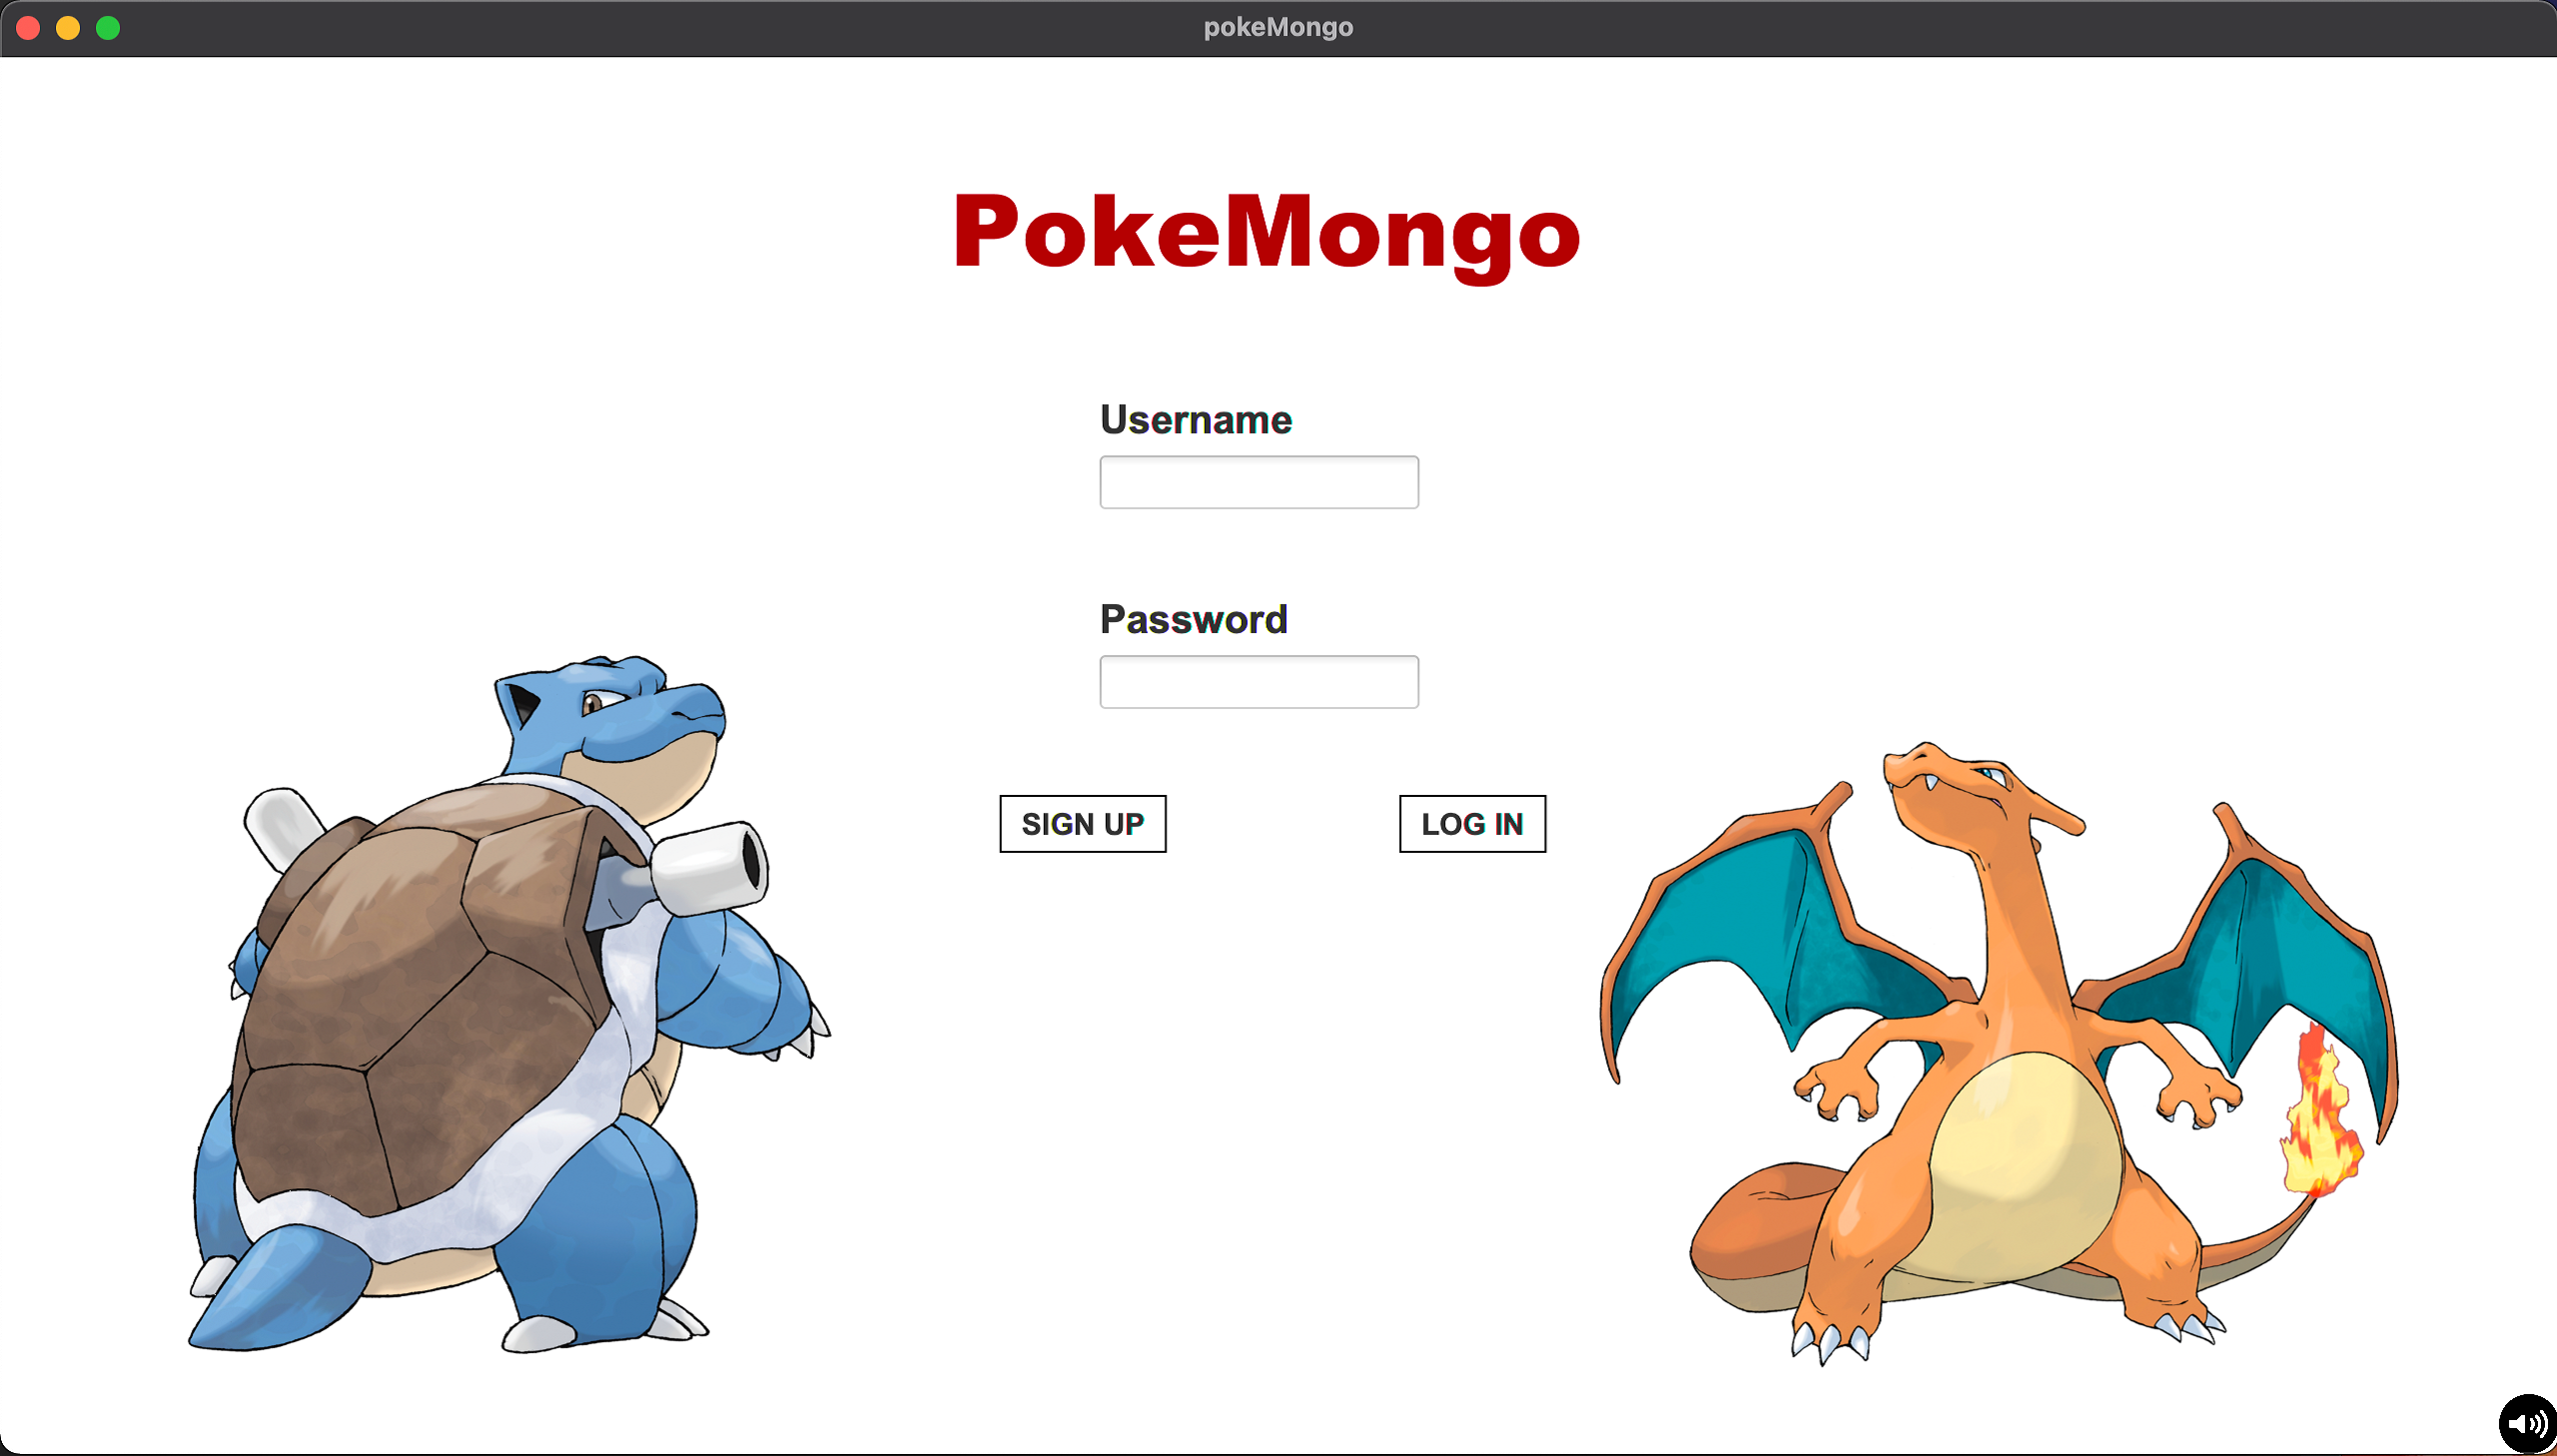
\includegraphics[width= \textwidth]{img/userManual/login.png}
	\caption{Login Page}
\end{figure}
The \textbf{User} must fill the textfields and press the \textbf{LOG IN button} in order to log in to the application or he can sign up to the service by pressing the \textbf{SIGN UP button}, compiling the registration form and then, pressing the \textbf{SUBMIT button}. If there are no errors, red popups won't be displayed. The \textbf{User} can turn back to the Login page by pressing the \textbf{BACK button}.
\begin{figure}[H]
	\centering
	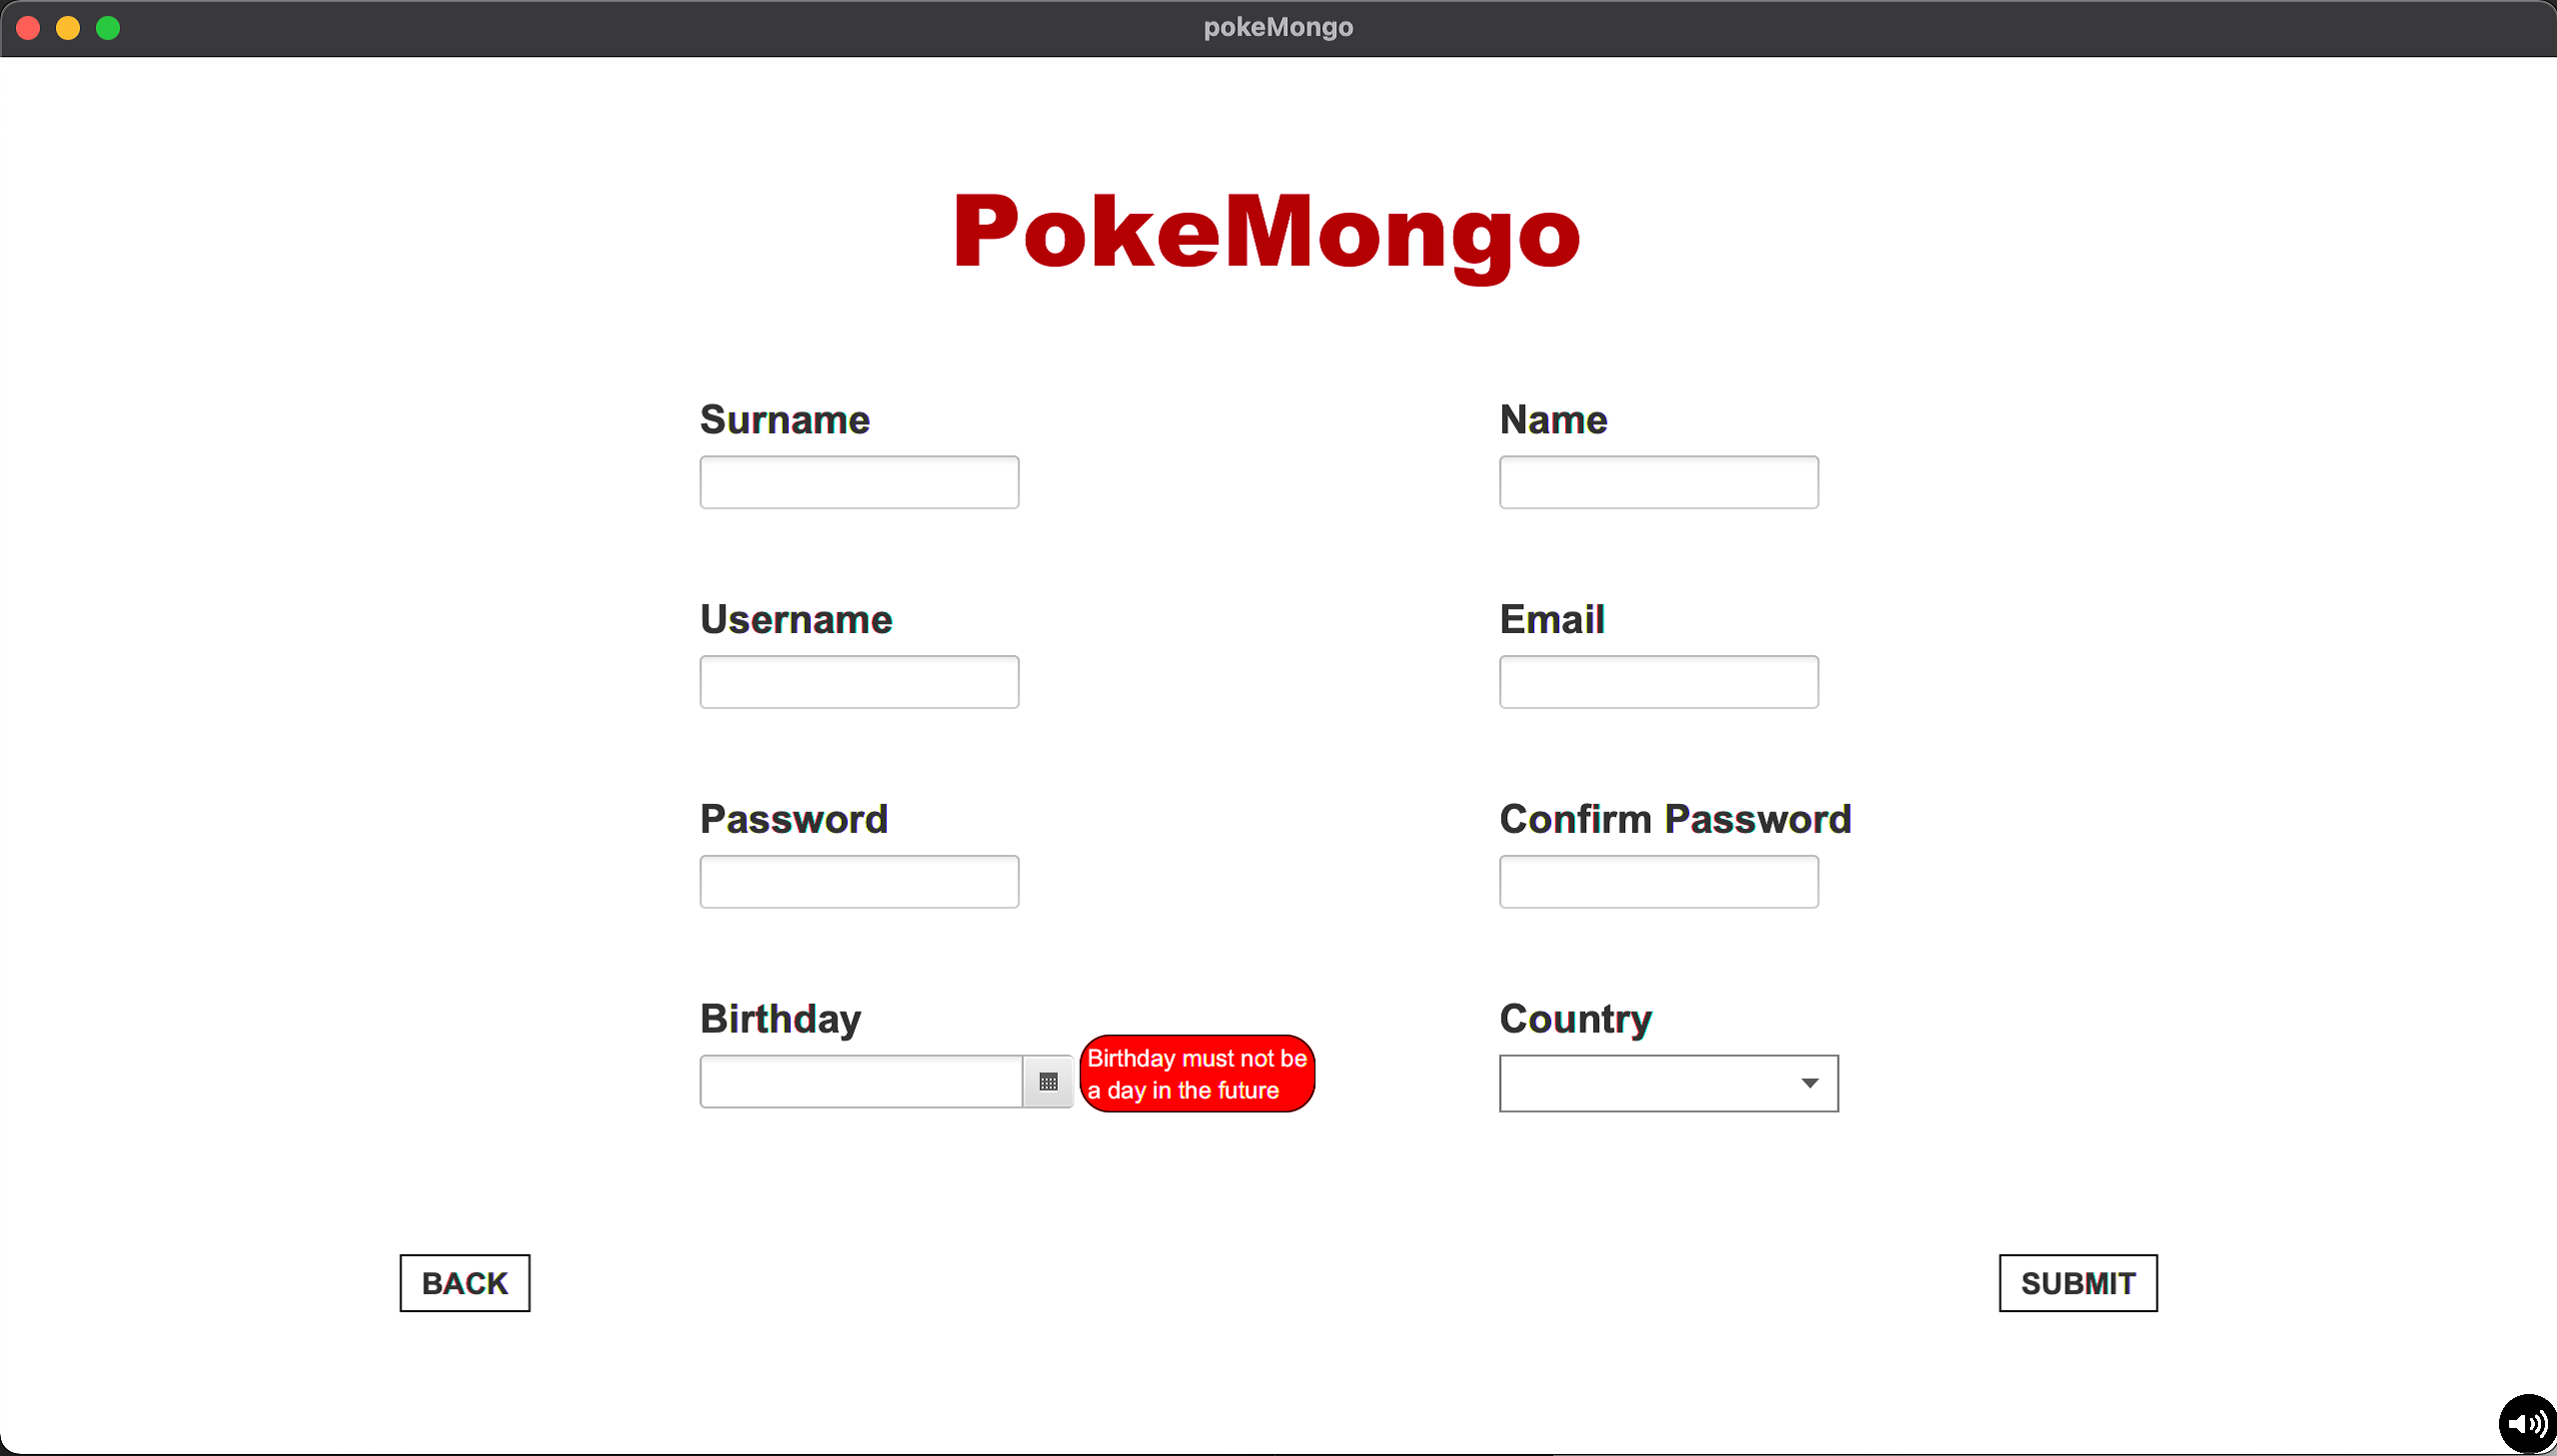
\includegraphics[width=\textwidth]{img/userManual/registration.png}
	\caption{Registration Page}
\end{figure}
The registration can only be made by \textit{Normal Users}, the \textit{Admins} credentials will be given to the client company.
After the login the following page will be displayed, in case of an \textit{Normal User}.
\begin{figure}[H]
	\centering
	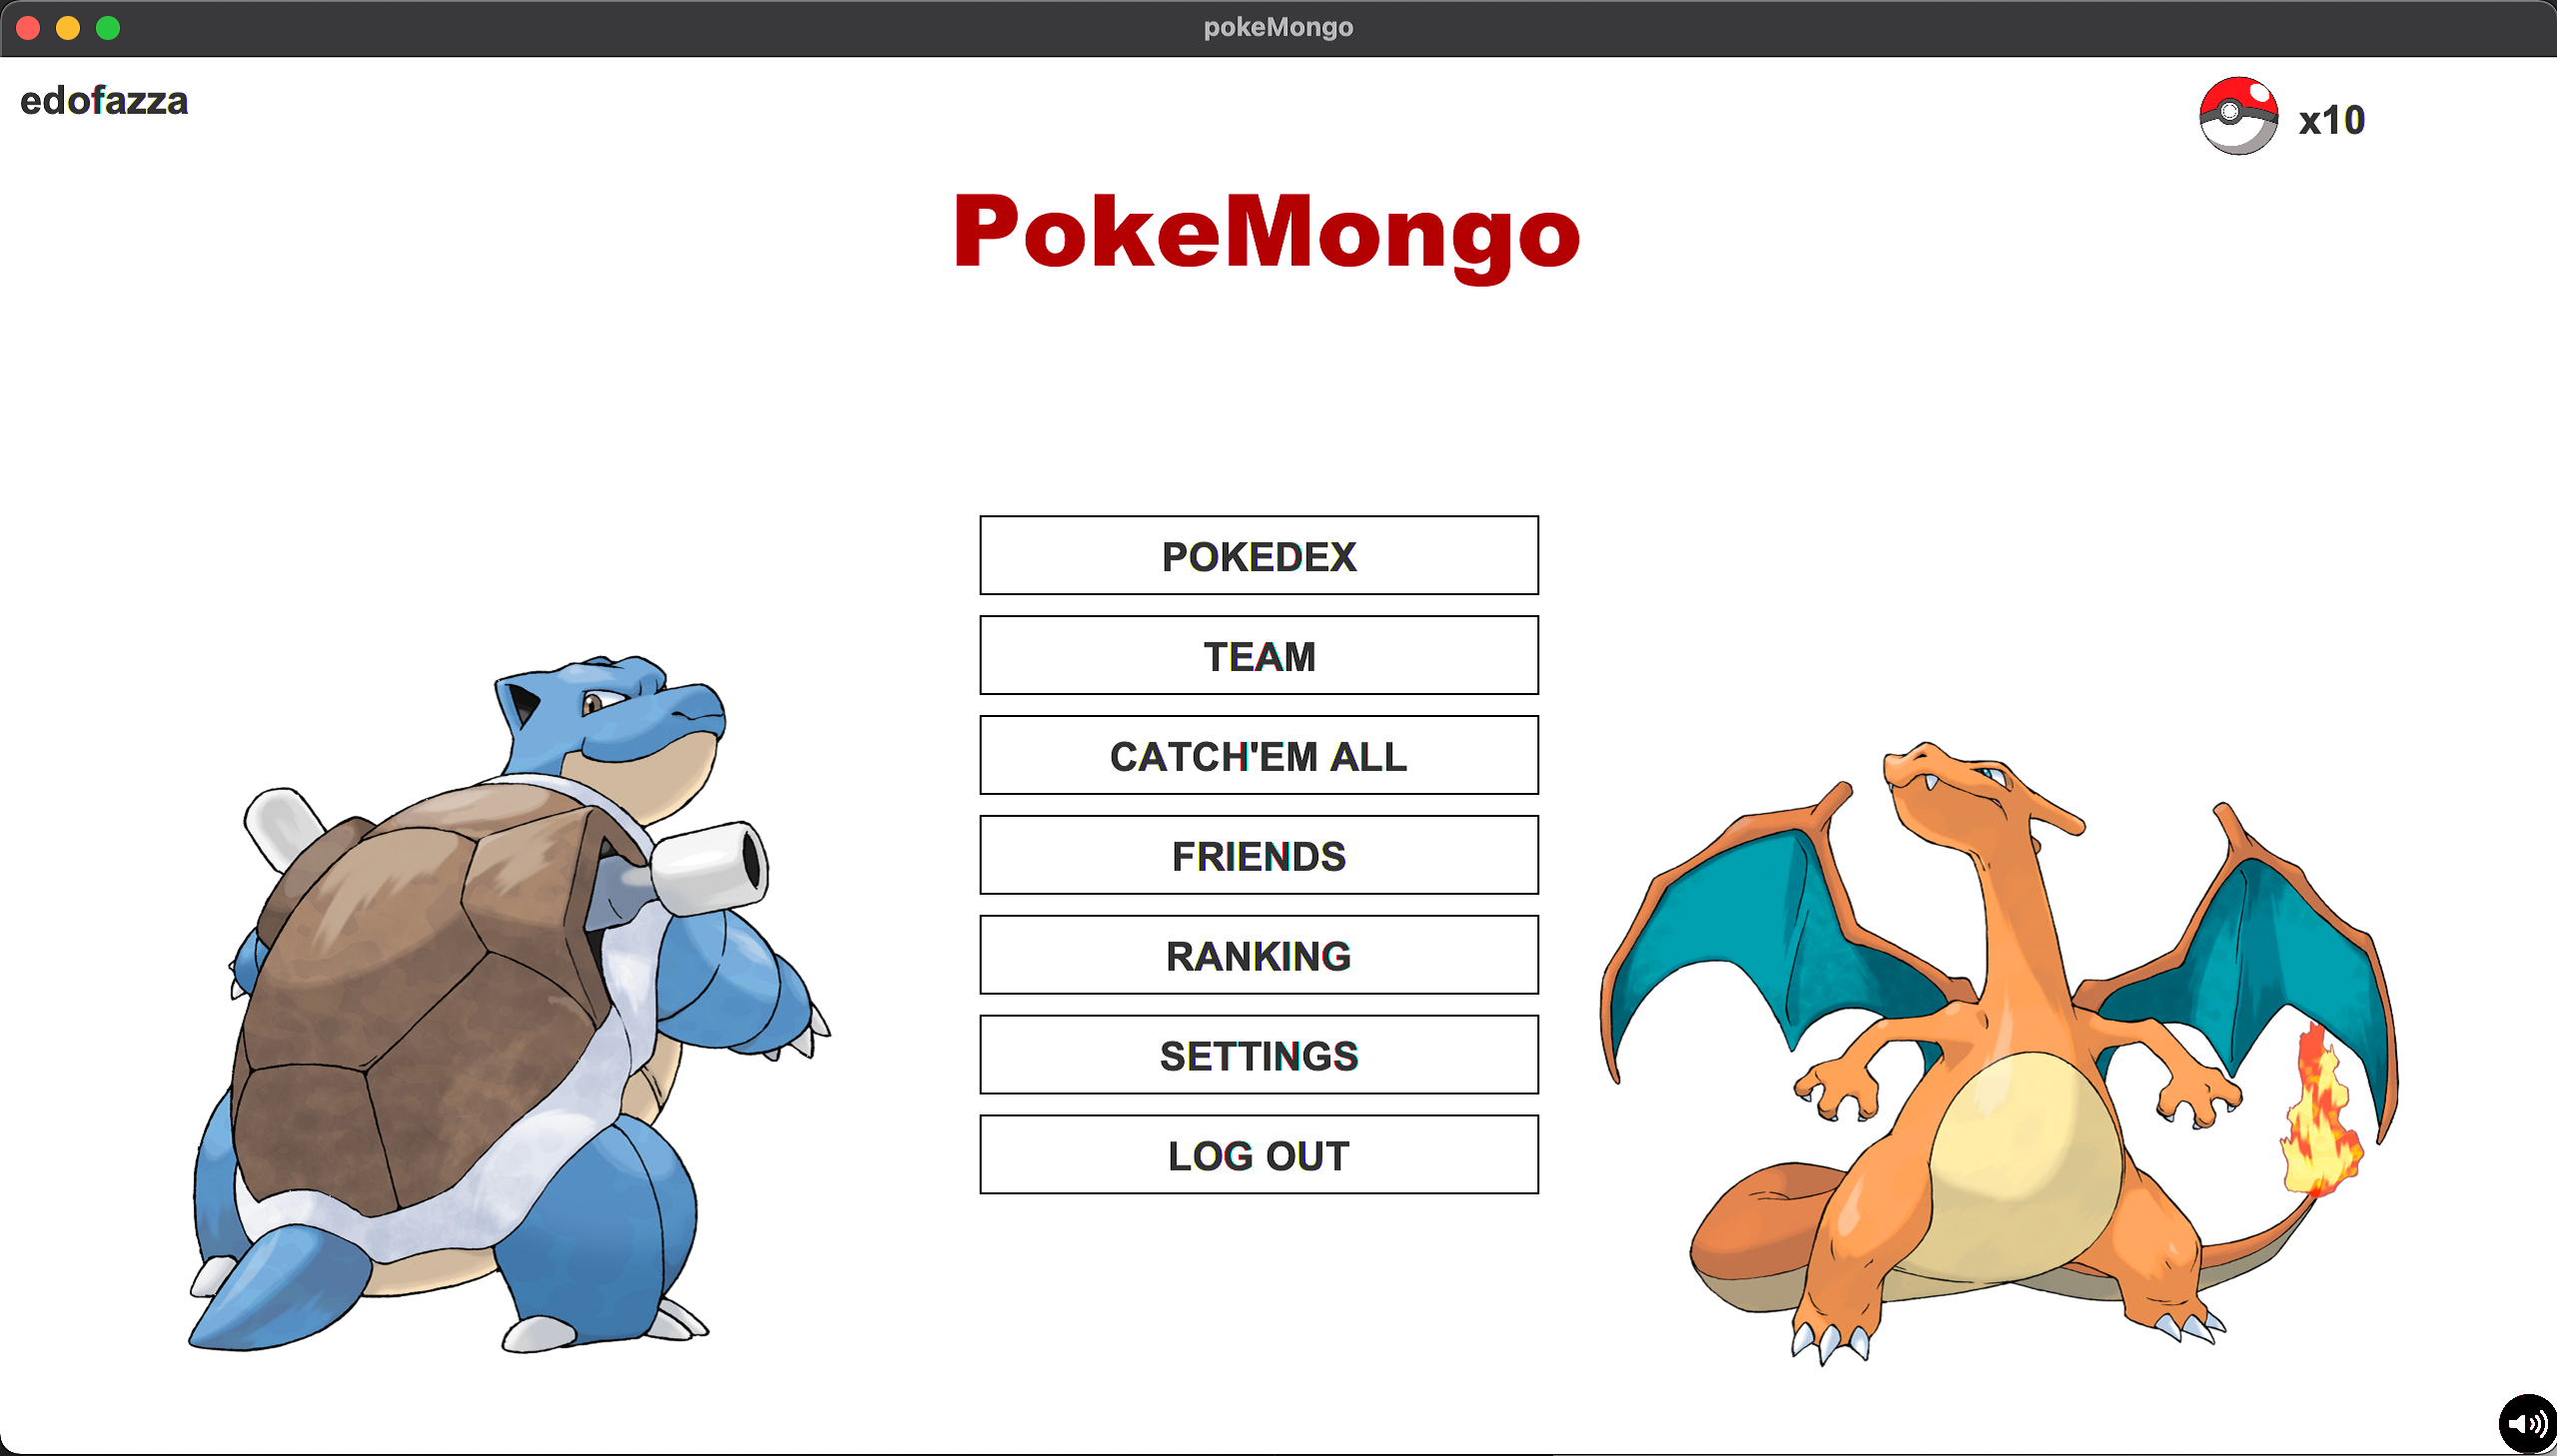
\includegraphics[width=\textwidth]{img/userManual/main.png}
	\caption{Normal User HomePage}
\end{figure}
We can notice that in the top-left corner is visible the \textit{username} whereas in the top-right corner the number of \textit{dailypokeball}. These items will be always visible when a user is logged to the application. On the bottom-right corner there is the \textbf{MUSIC button} which, if pressed, will stop the music played at the launch of the application.

\subsubsection{Pokedex}
The \textit{Pokedex} will help the \textbf{User} to discover new \textbf{Pokemons} and to know more about them.
\begin{figure}[H]
	\centering
	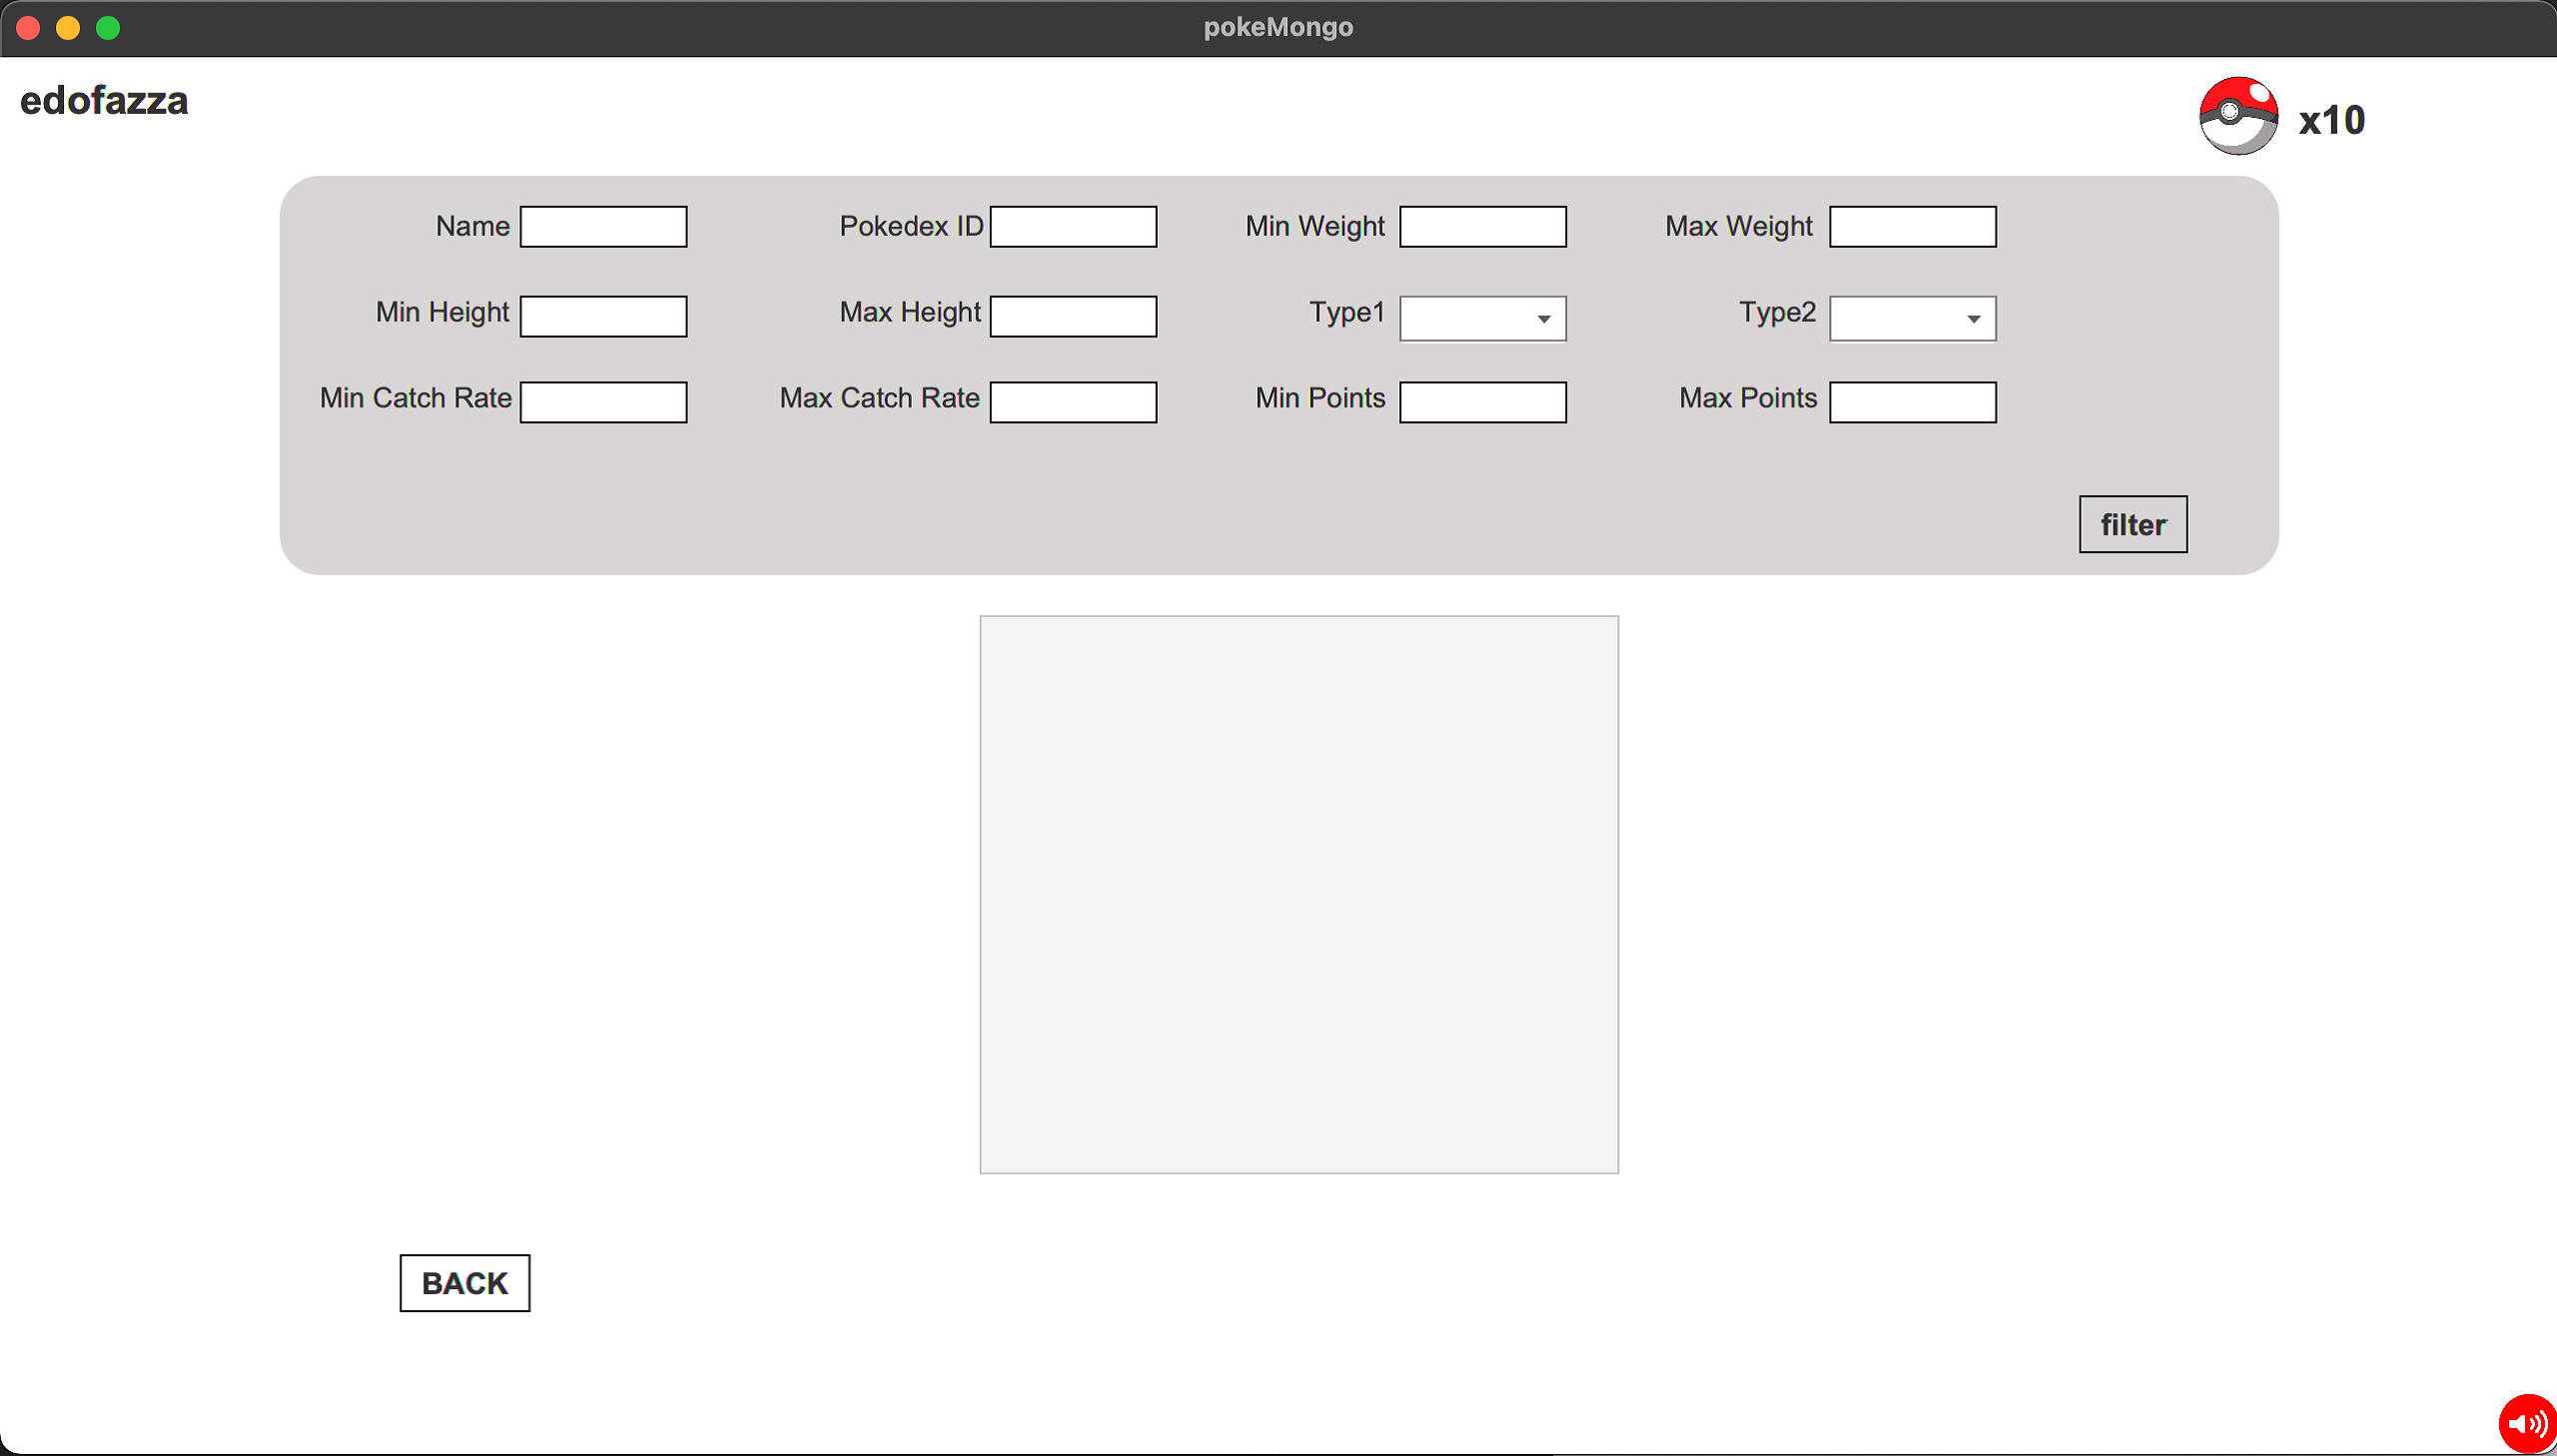
\includegraphics[width=\textwidth]{img/userManual/pokedex.png}
	\caption{Pokedex Page}
\end{figure}

The \textbf{User} can set as many parameters as he want for searching but at least one should be set. After setting some filters the \textbf{User} must click the \textbf{FILTER button} in order to get the search results. In the following image there is an example of the  of the \textit{Pokedex} page.
\begin{figure}[H]
	\centering
	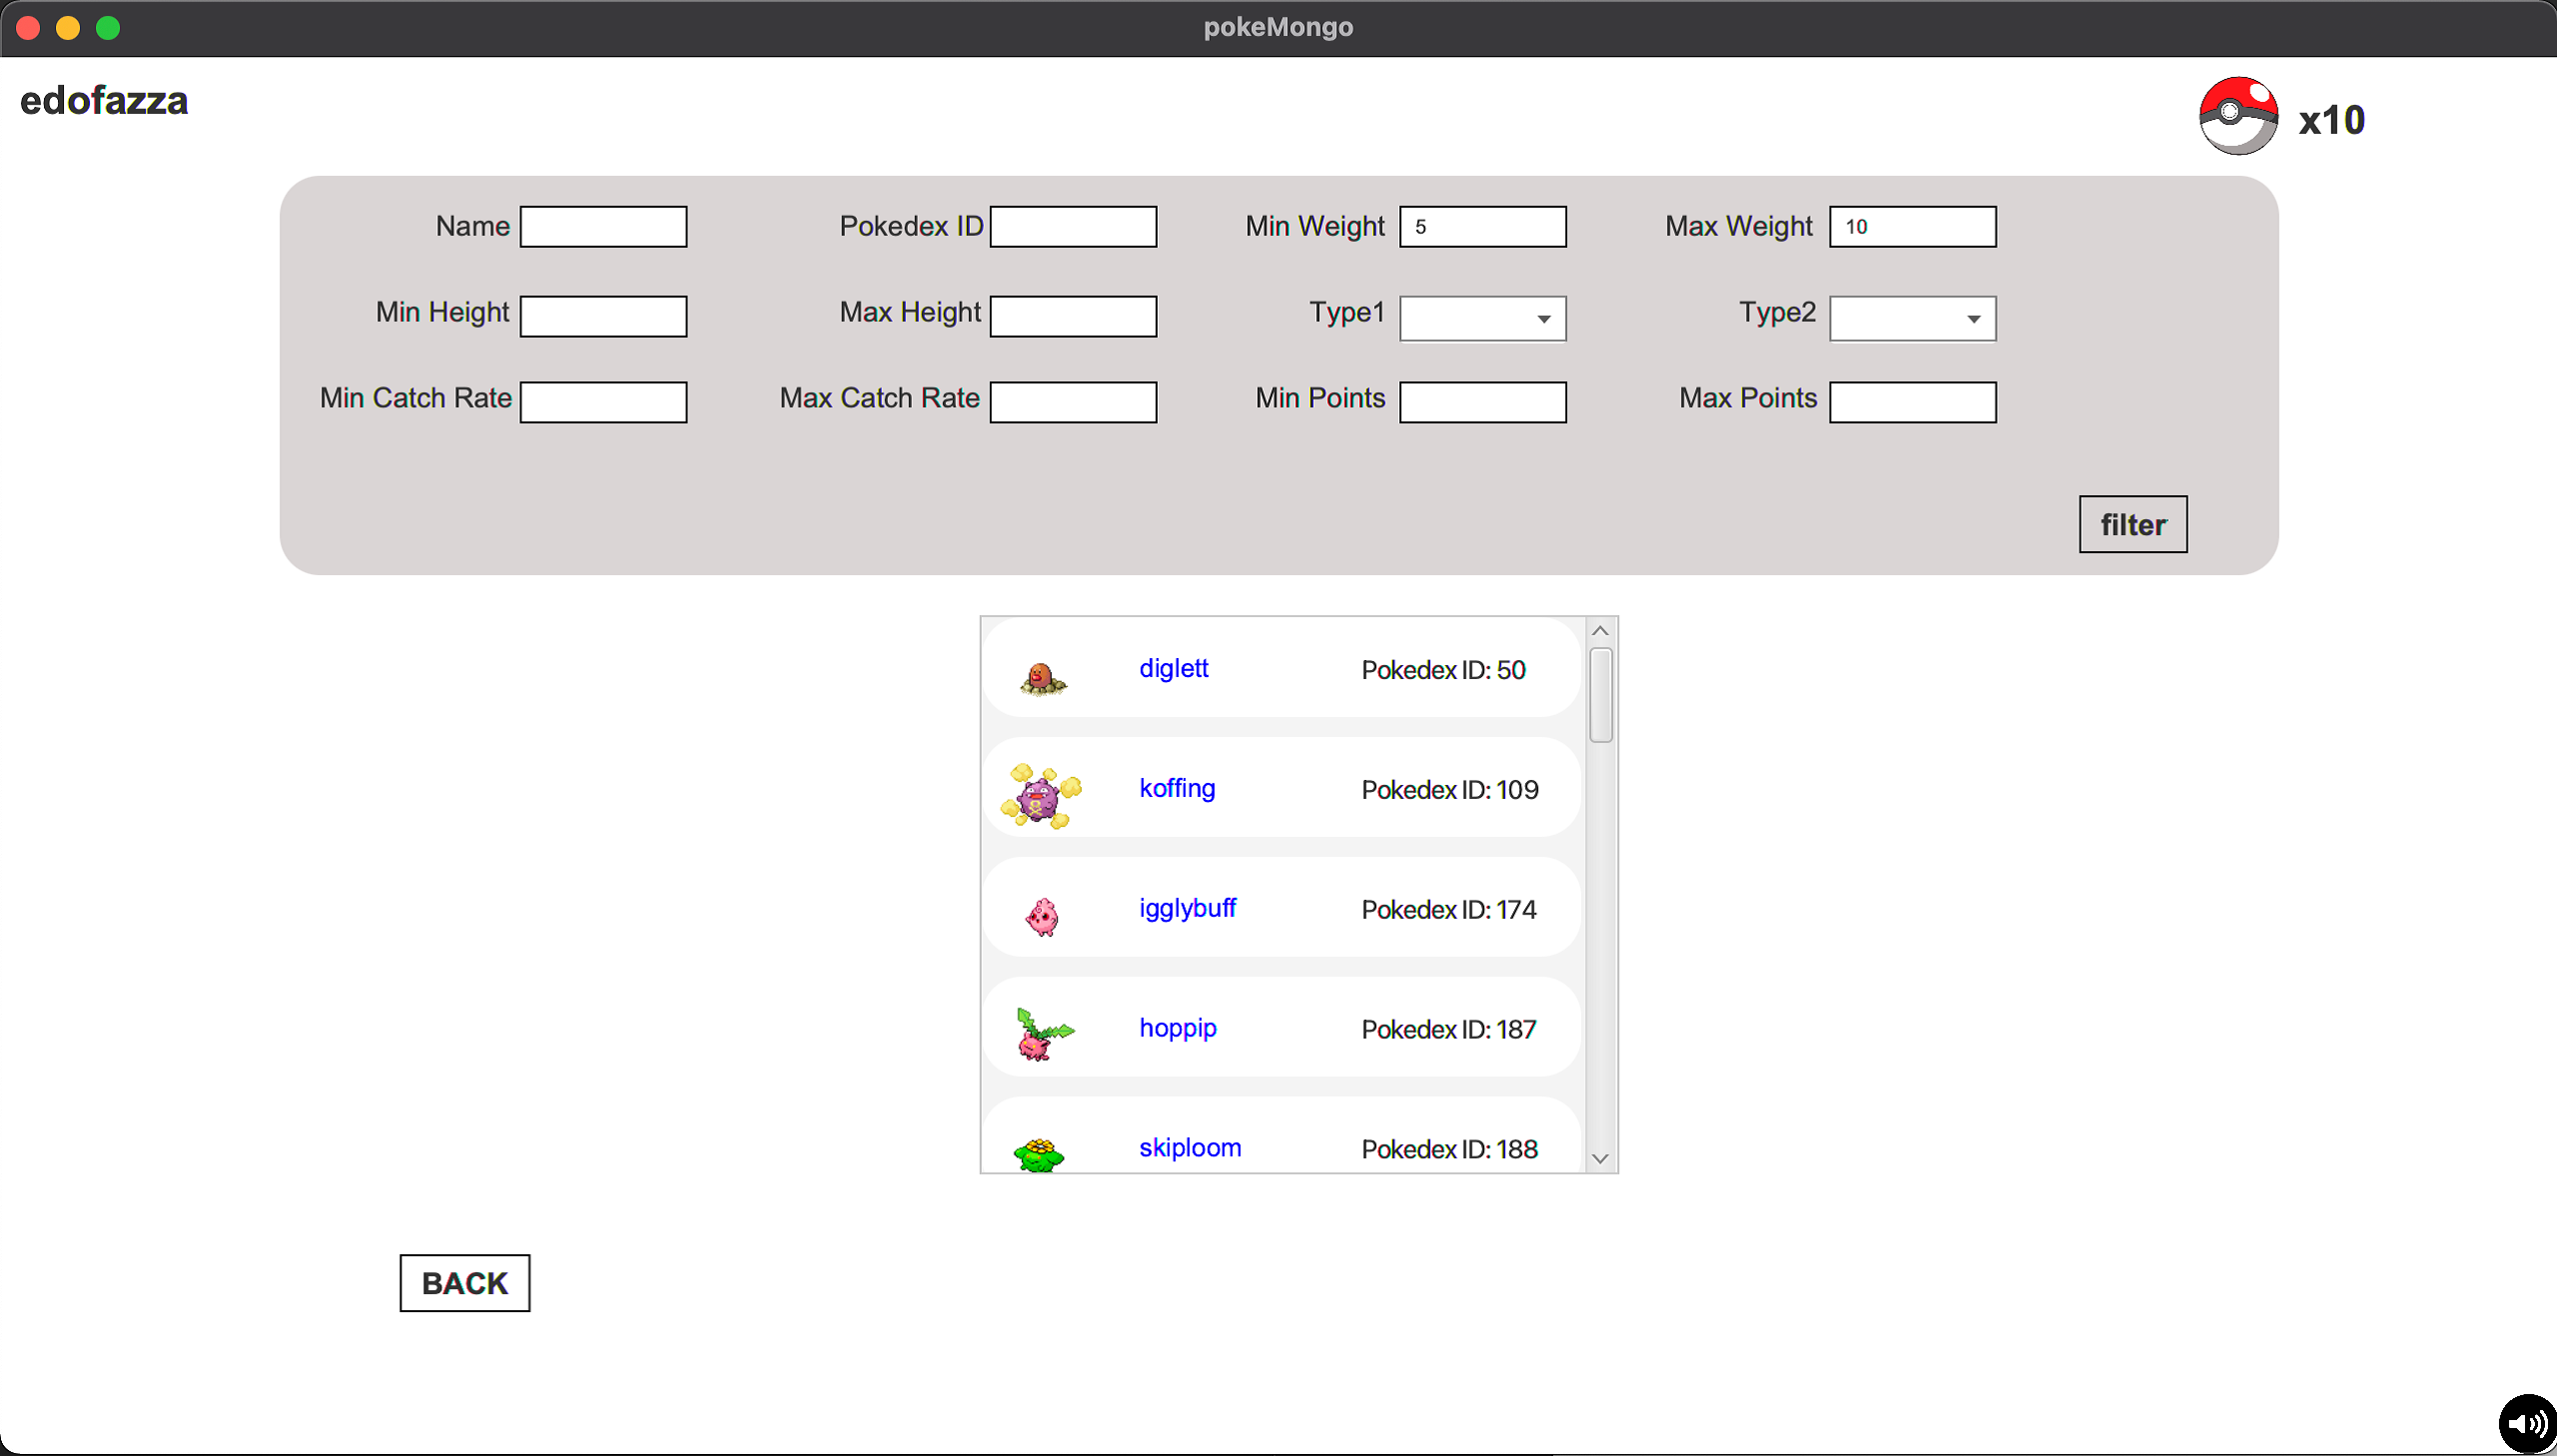
\includegraphics[width=\textwidth]{img/userManual/pokedex2.png}
	\caption{Pokedex Page after filtering}
\end{figure}
\textbf{Notice that if there is no internet connection, no image will be loaded, but the application will still work.} The \textbf{BACK button} will redirect again to the \textit{Normal User Homepage}. If the \textbf{User clicks} on the name of the \textbf{Pokemon}, a popup will be shown. 
\begin{figure}[H]
	\centering
	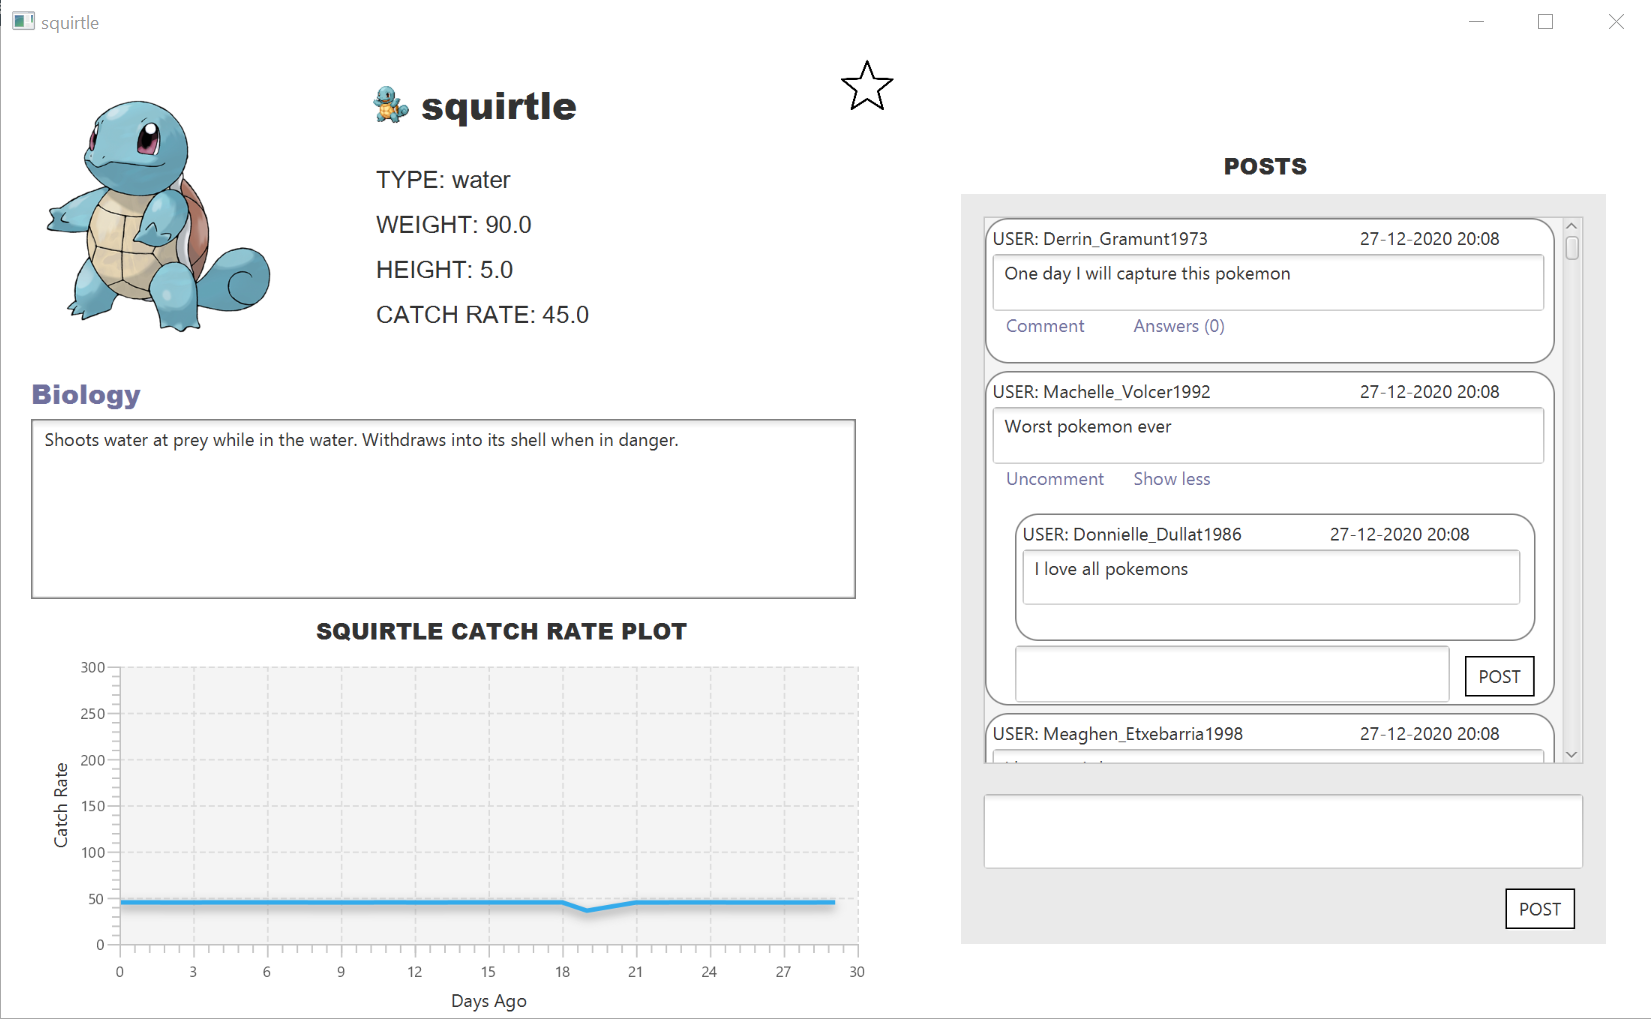
\includegraphics[width=\textwidth]{img/userManual/pokemon_info.png}
	\caption{Pokemon Info's Window}
\end{figure}
In the popup all the information regarding a single \textbf{Pokemon} will be displayed. At the left bottom corner there is a plot in which it’s displayed the evolution of the catch rate of selected \textbf{Pokemon} in the last thirty days. The \textbf{STAR button} is a special button, if the \textbf{User} clicks on it that \textbf{Pokemon} will be added to the favourite ones. By clicking on the button the star will turn yellow. To remove the \textbf{Pokemon} from favourites the \textbf{User} must click on it another time. Then, the star will turn than white again.\\
On the right there is the \textit{Post Section} where the \textbf{User} can write a \textbf{Post} about the \textbf{Pokemon} viewed or reply to other \textbf{Posts}. If the \textbf{User} is the creator of a \textbf{Post} he can delete it by just clicking on the red \textbf{DELETE writing} inside the \textbf{Post} or the \textbf{Reply}.
\subsubsection{Team}
The \textit{Team page} lets the \textbf{User} handle his personal \textbf{Team}.
There will be displaye the \textbf{captured Pokemons}. 
\begin{figure}[H]
	\centering
	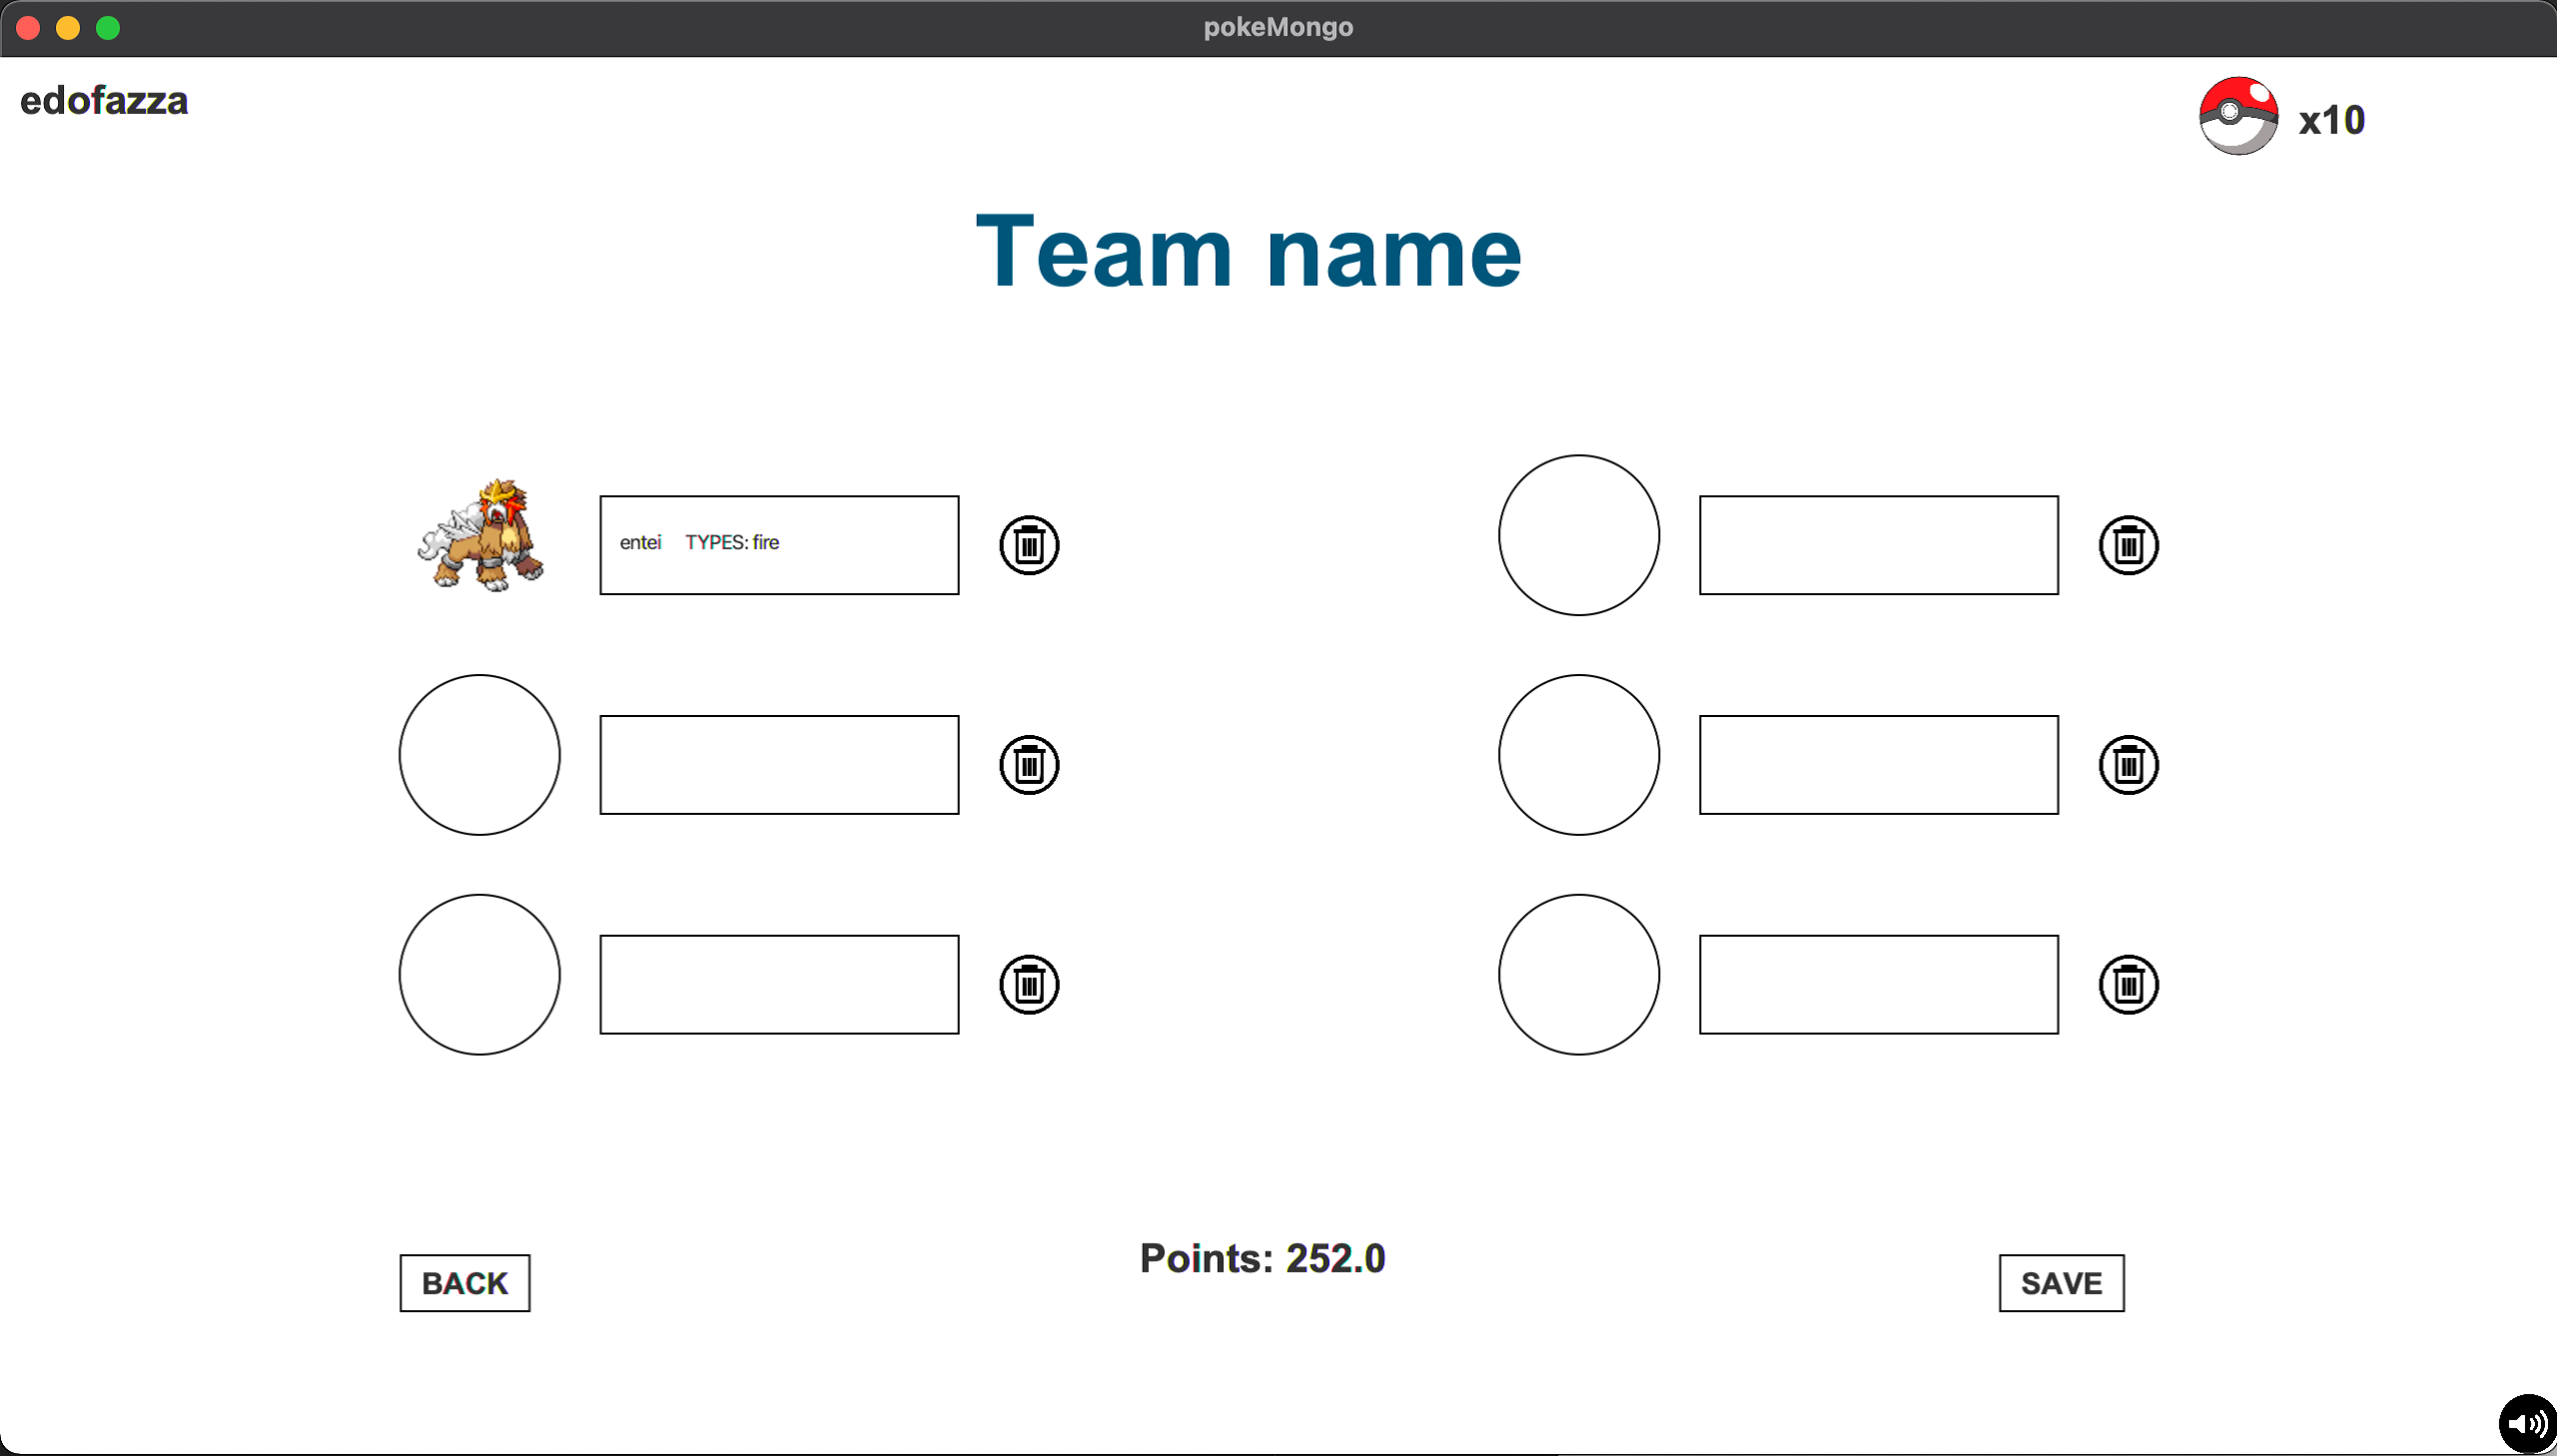
\includegraphics[width=\textwidth]{img/userManual/team.png}
	\caption{Team Page}
\end{figure}
The \textbf{TRASH button} near the \textit{slot} can eliminate the \textbf{Pokemon} from the \textbf{Team} (don’t worry! The User won’t kill it, he’ll just free it). The \textit{Team name} is displayed at the top and it is editable. At the bottom are shown the \textit{team points}. Any changes in the \textbf{Team} must be saved to completely store them in a persistent way, to do so the \textbf{User} must \textit{press} the \textbf{SAVE button}.

\subsubsection{Catch'em All}
In the \textit{Catch'em All Page} the \textbf{User} can capture other \textbf{Pokemons}. In order to do so the \textbf{User} must type the \textit{Pokemon name} or \textit{click} on one field of the favourite table on the right in order to copy quickly the name of a favourite one. Then, he must choose a \textit{slot} to capture the \textbf{Pokemon}, where this \textit{slot} must be free, and, at the end, he must \textit{click} the \textbf{TRY TO CATCH button} in order to make the capture attempt, which success will depend on the odd (the capture rate percentage) of the \textbf{Pokemon}. The result of the attempt will be shown below. The \textbf{User} has a limited number of \textit{pokeballs} (for instance, 10 pokeballs per day), which represent the number of possible attempts to capture a Pokemon. If no pokeballs are left the \textbf{User} can't perform the capture attempt.
\begin{figure}[H]
	\centering
	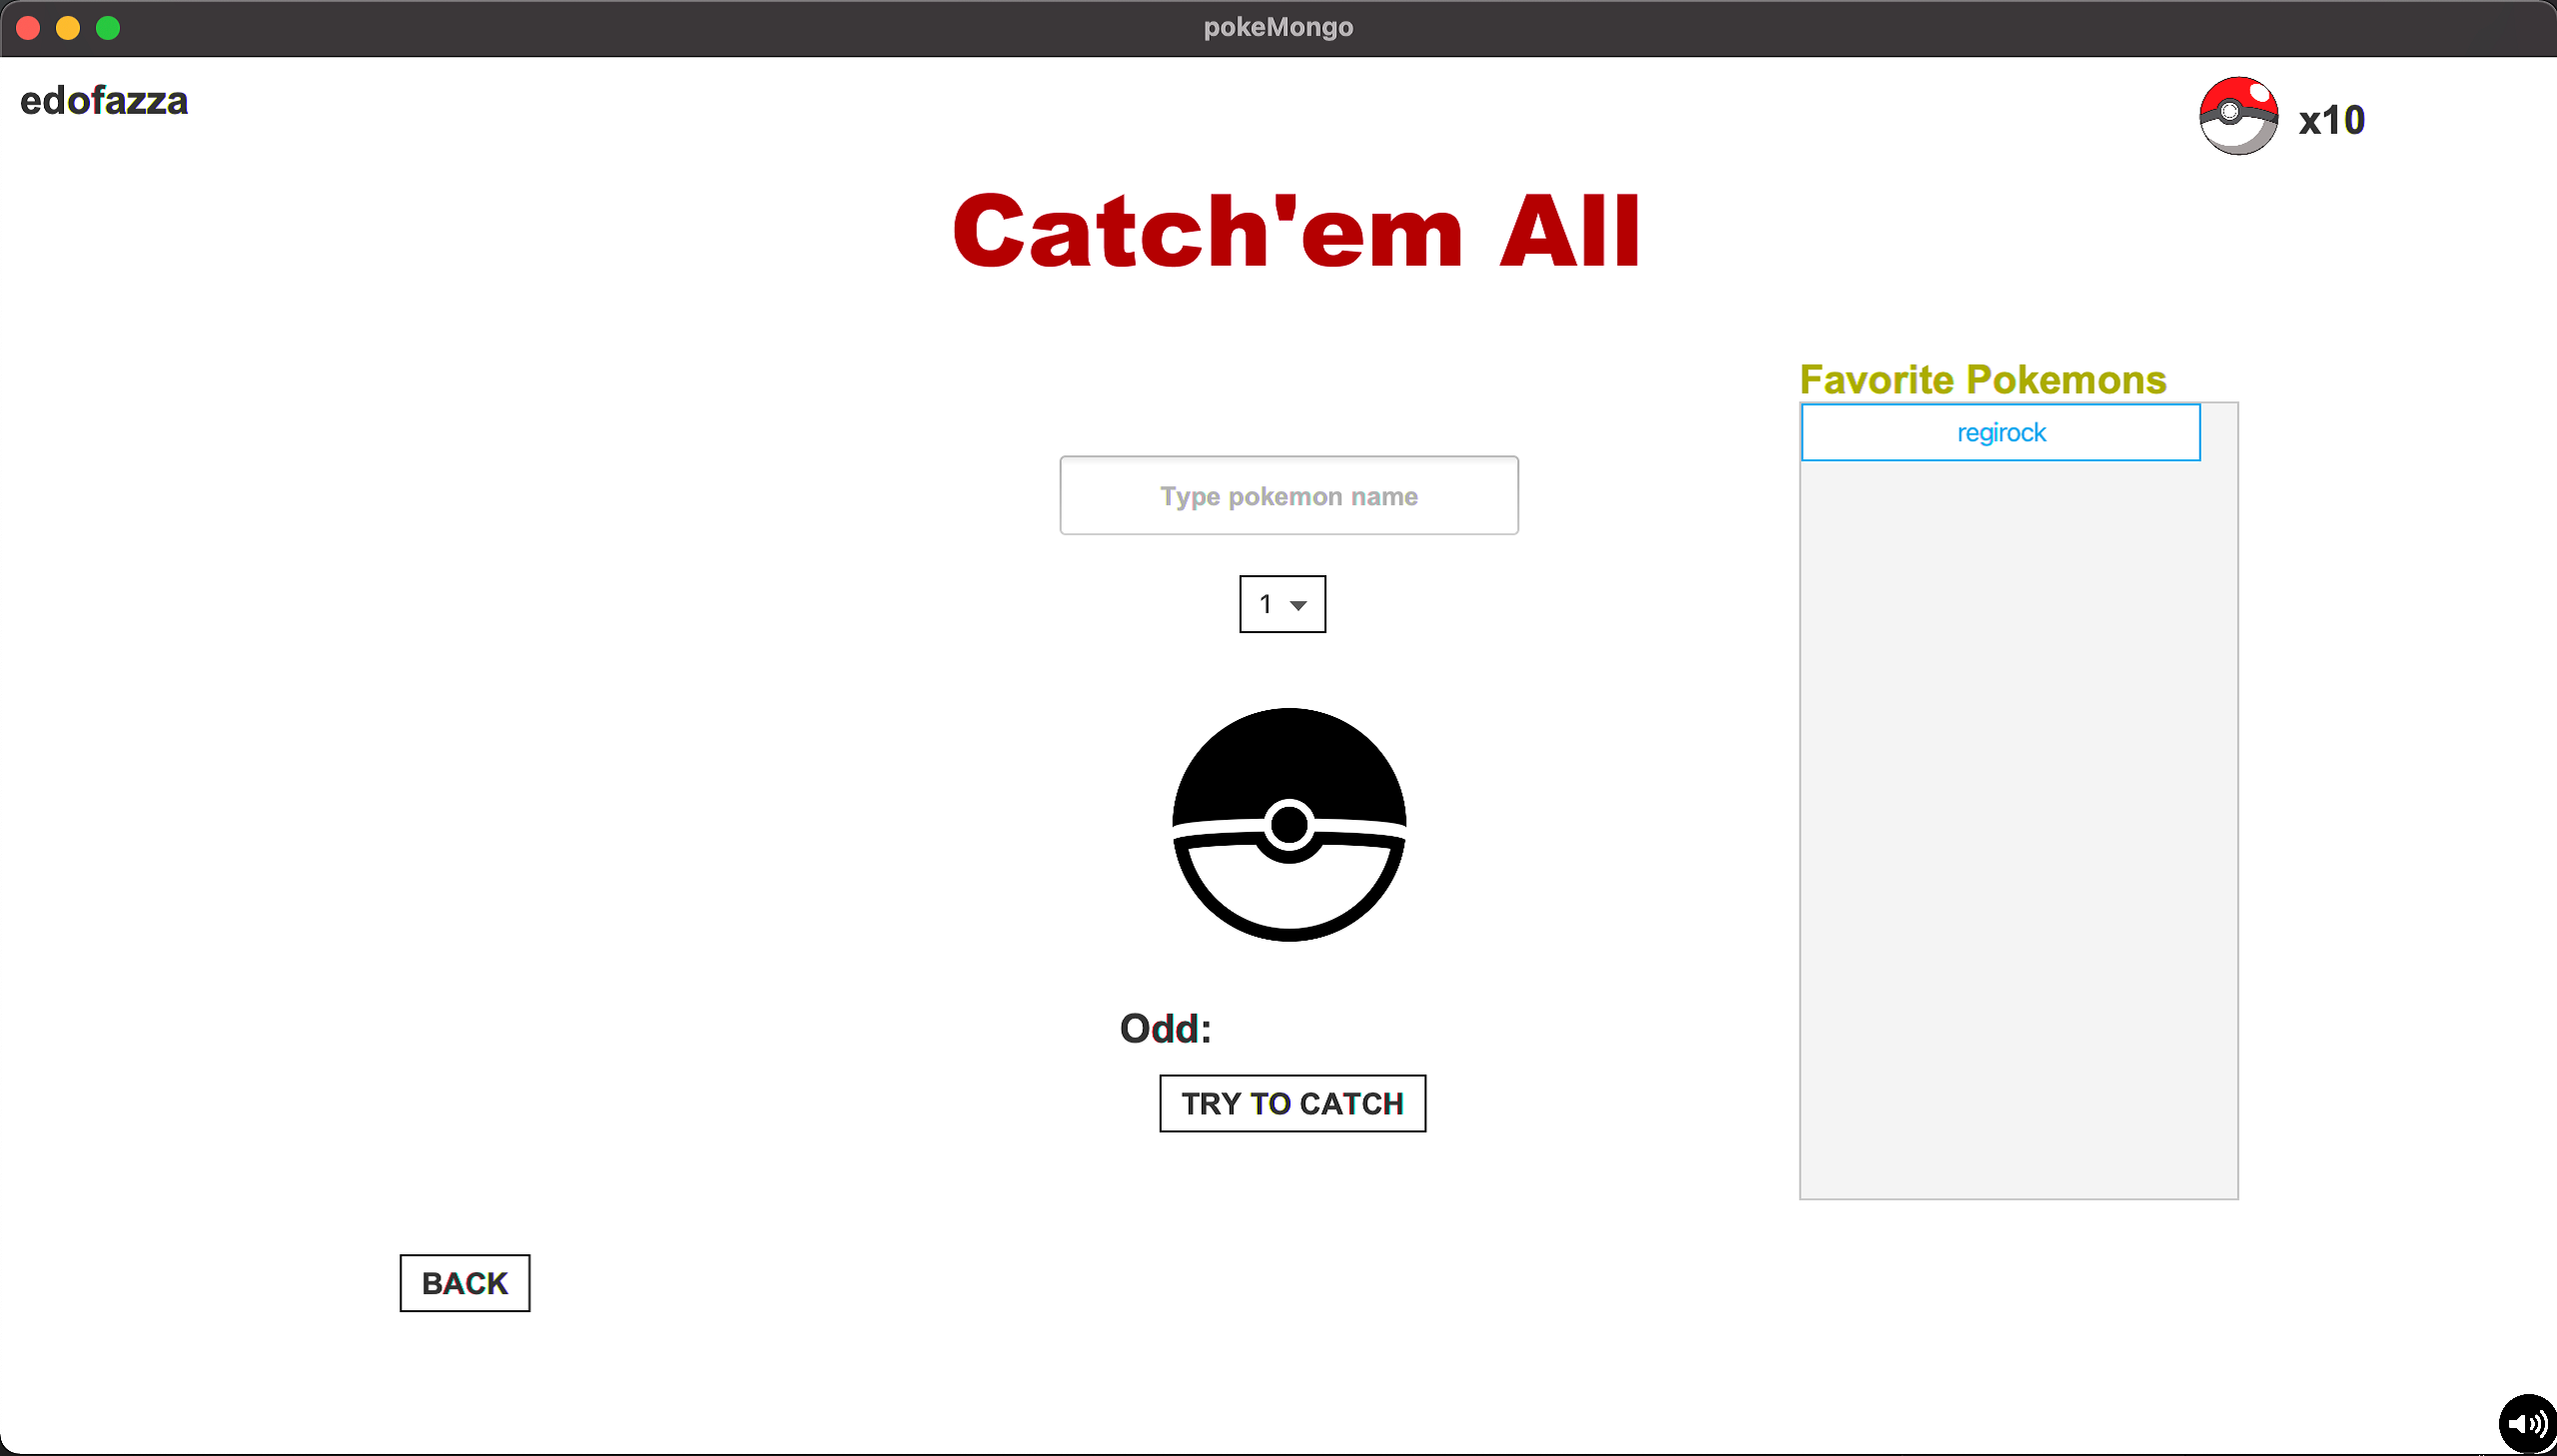
\includegraphics[width=\textwidth]{img/userManual/catch.png}
	\caption{Catch'em All Page}
\end{figure}
\subsubsection{Friends}
In the \textit{Friends Page} are shown information about the friends, people who the \textbf{User} follows, of a \textbf{User}. 
\begin{figure}[H]
	\centering
	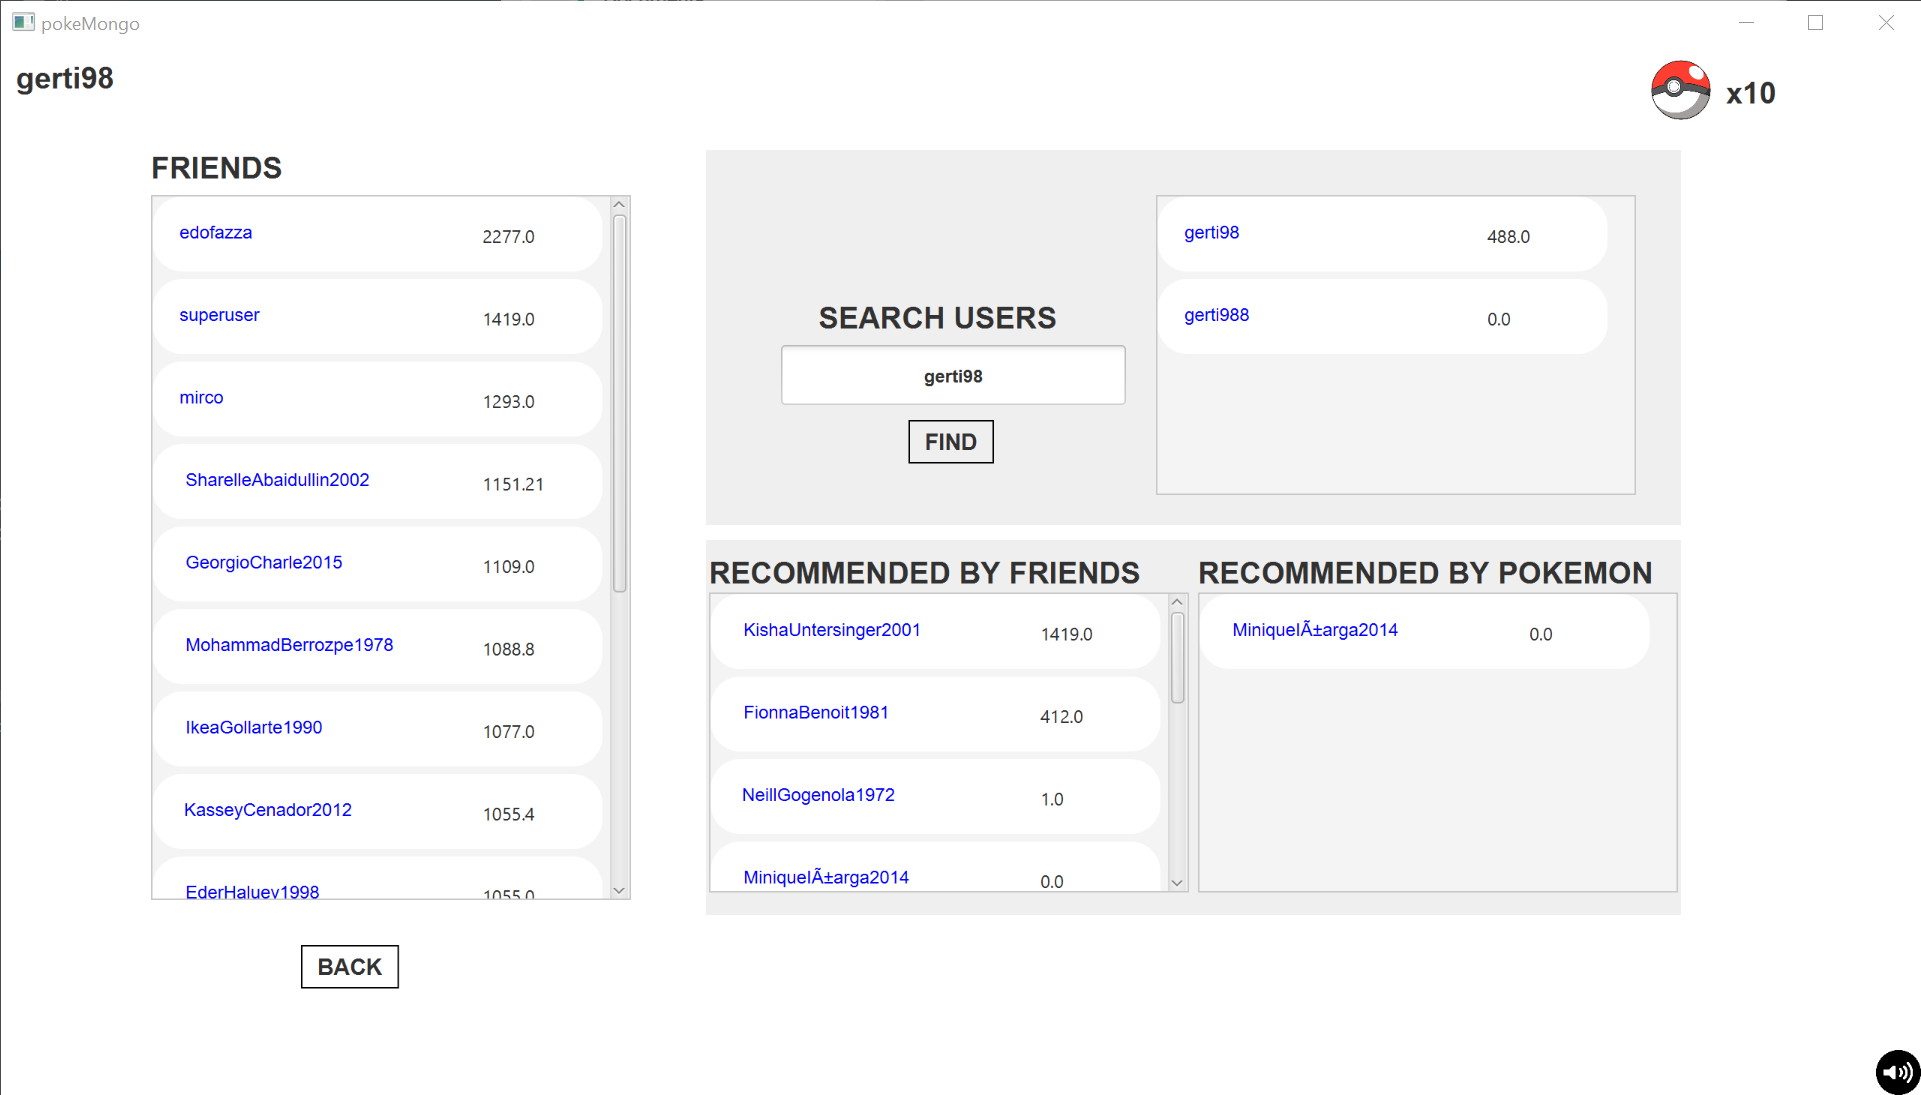
\includegraphics[width=\textwidth]{img/userManual/friends.png}
	\caption{Friends Page}
\end{figure}
In the left pane is displayed the friends list of the \textbf{User}, in the top-right pane is possible to search a particular \textbf{User} by \textit{username}, whereas, in the bottom-left panes, are shown some suggested \textbf{Users} to follow based on the people followed or the pokemon liked by the \textbf{User}.
By clicking on a \textit{username} will be shown another popup. In the following image it is showed:
\begin{figure}[H]
	\centering
	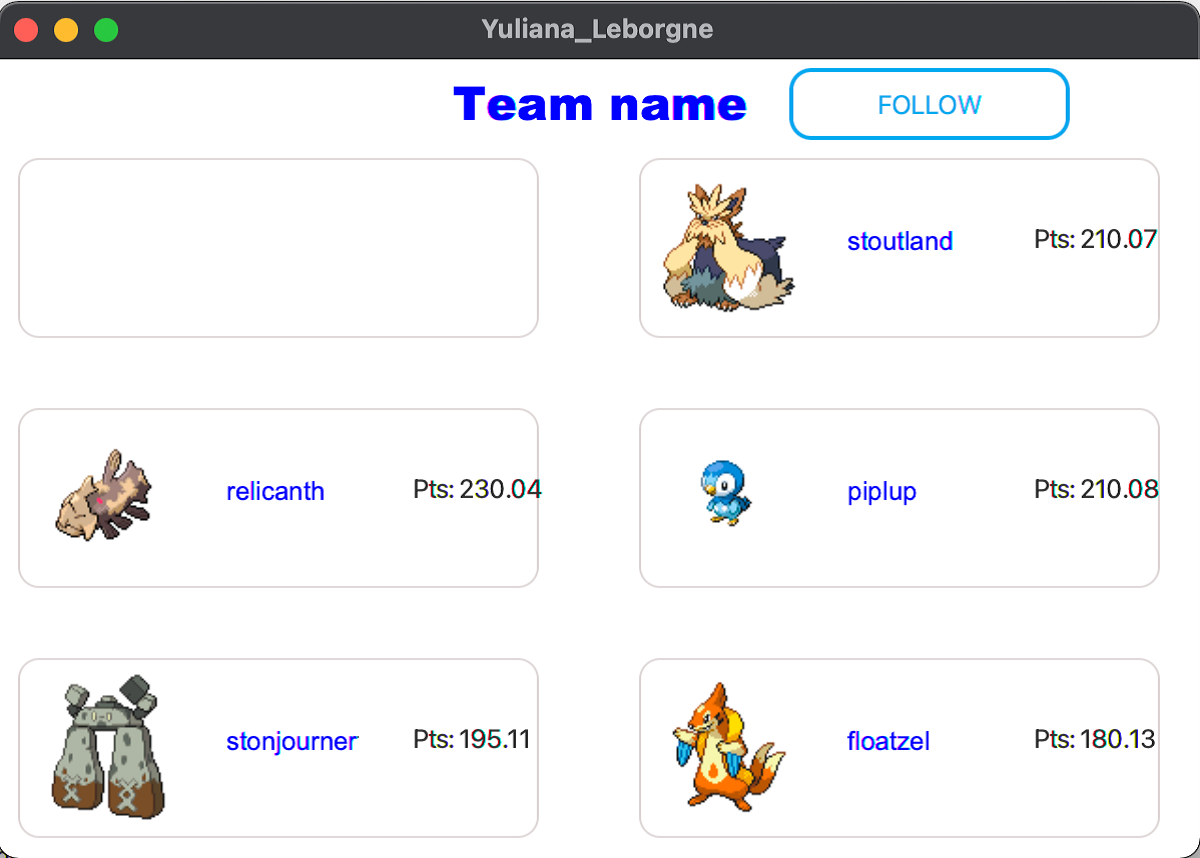
\includegraphics[width=\textwidth]{img/userManual/team_popup.png}
	\caption{User Team Popup}
\end{figure}
In which the \textbf{Team} composition and the \textit{team name} of a particular \textbf{User} is displayed. By \textit{pressing} the \textbf{FOLLOW button}, at the top right corner, that particular \textbf{User} is added to the friends list and the button will turn into an \textbf{UNFOLLOW button}, which, of course, will permit to delete a \textbf{User} from the friends list.
\subsubsection{Ranking}
In this page are displayed different types of ranking: the \textit{Most Used Pokemon} and the \textit{Best Teams}, which can be filtered by \textit{Country}, and the \textit{Best Teams among friends}. In the following image is shown how this page is displayed in the application:
\begin{figure}[H]
	\centering
	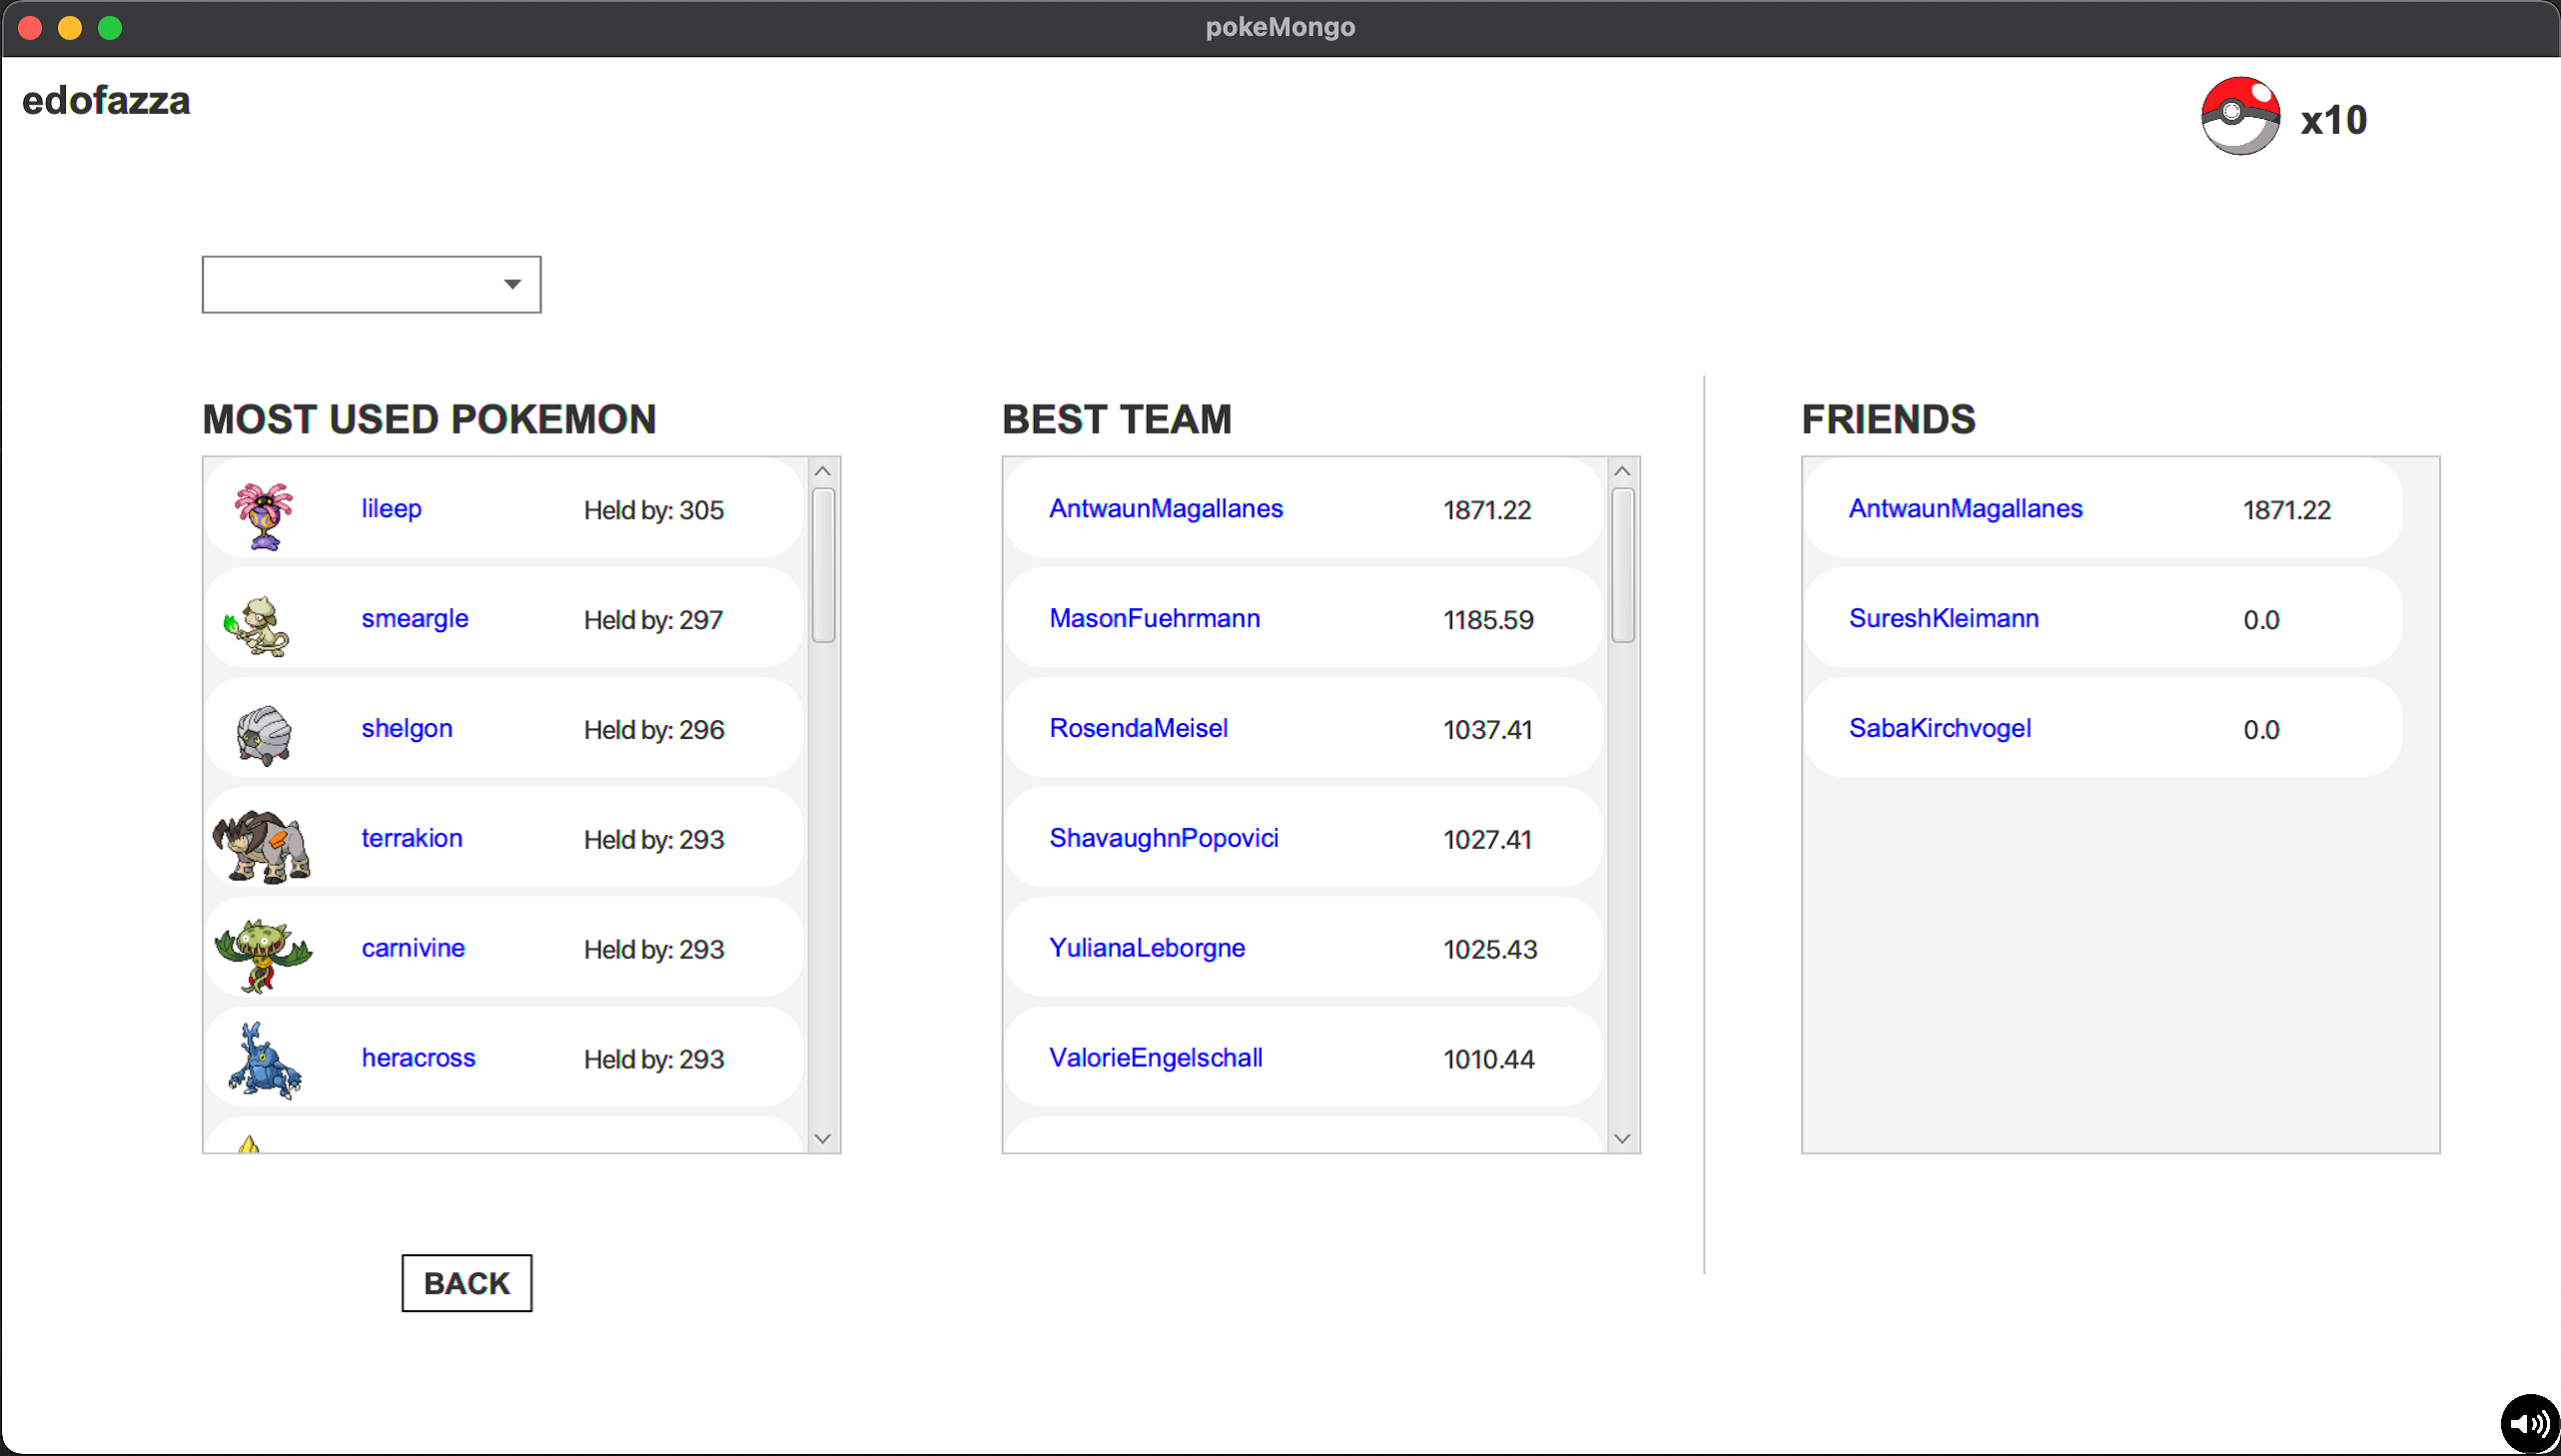
\includegraphics[width=\textwidth]{img/userManual/ranking.png}
	\caption{Ranking Page}
\end{figure}
By \textit{clicking} on the top-left combobox is possible to perform the \textit{Country} filtering of the Rankings (the friens one won't be affected).

\subsubsection{Settings}
In this page is possible to modify some \textbf{User} registration information like the \textit{email}, the \textit{password} and the \textit{country}.
\begin{figure}[H]
	\centering
	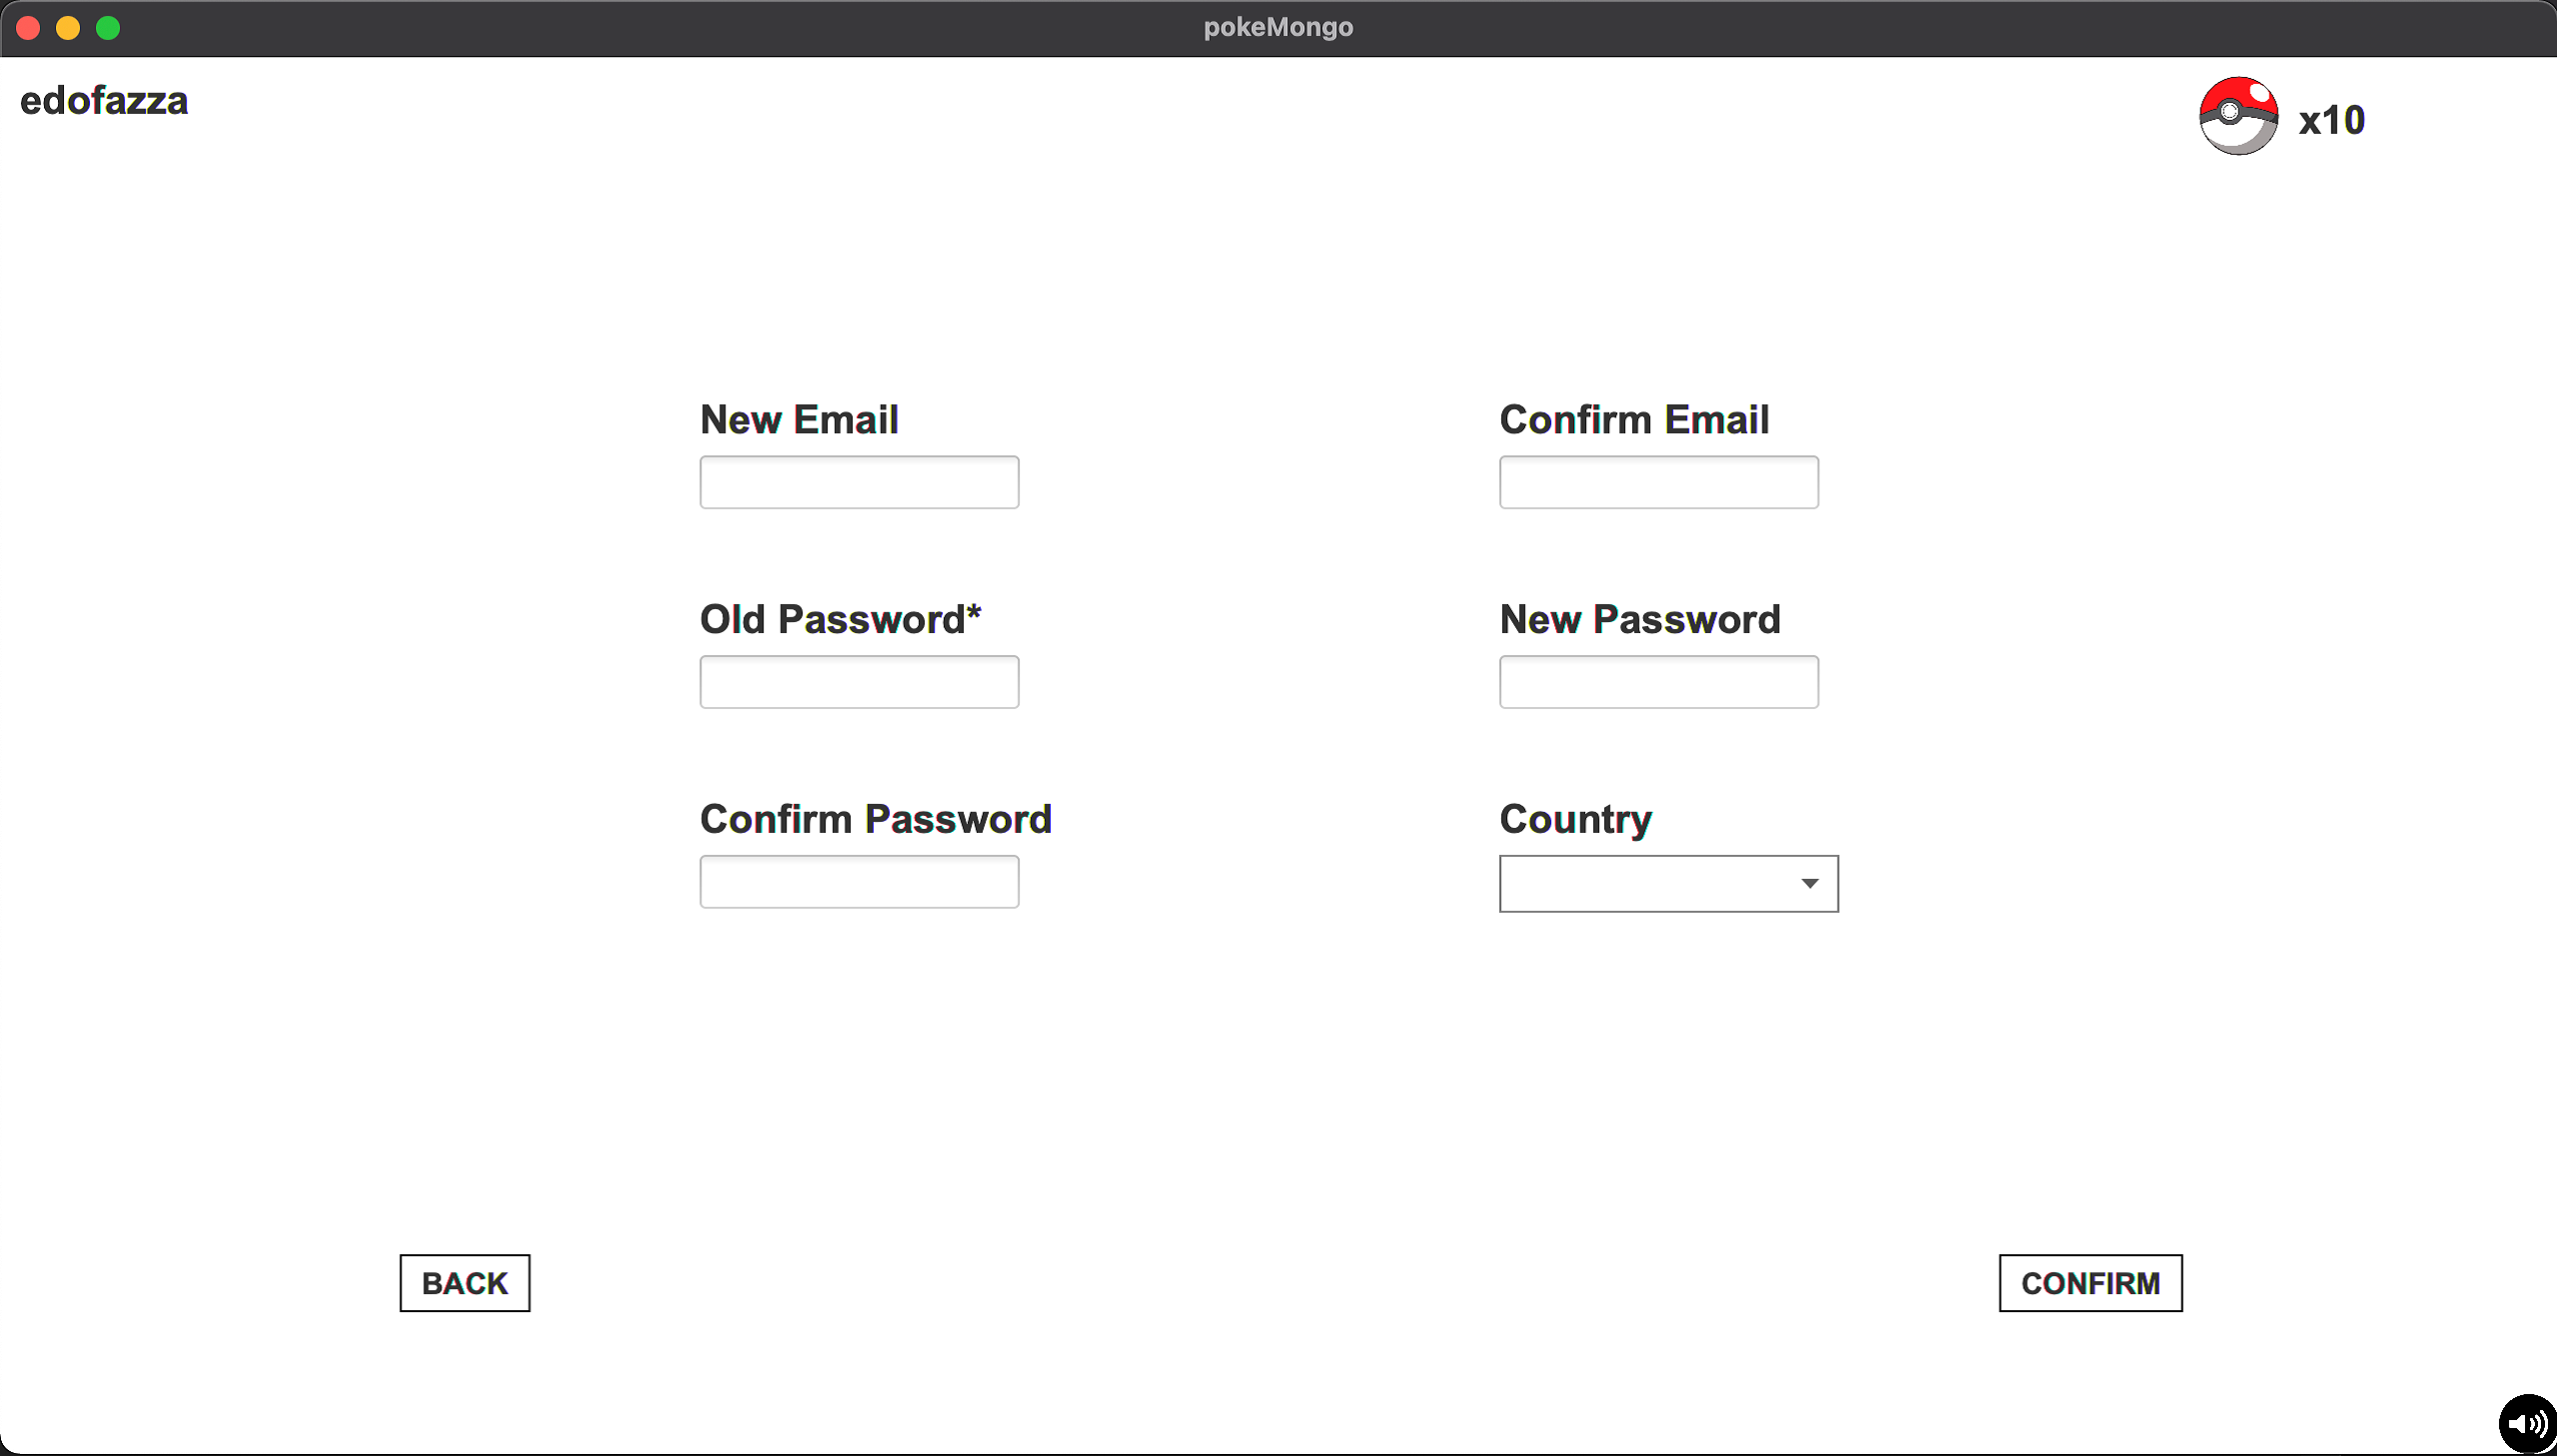
\includegraphics[width=\textwidth]{img/userManual/settings.png}
	\caption{Settings Page}
\end{figure}
\subsection{Admin Manual}
\subsubsection{Admin Homepage}
After the login of the \textbf{Admin} the following homepage will be shown.
\begin{figure}[H]
	\centering
	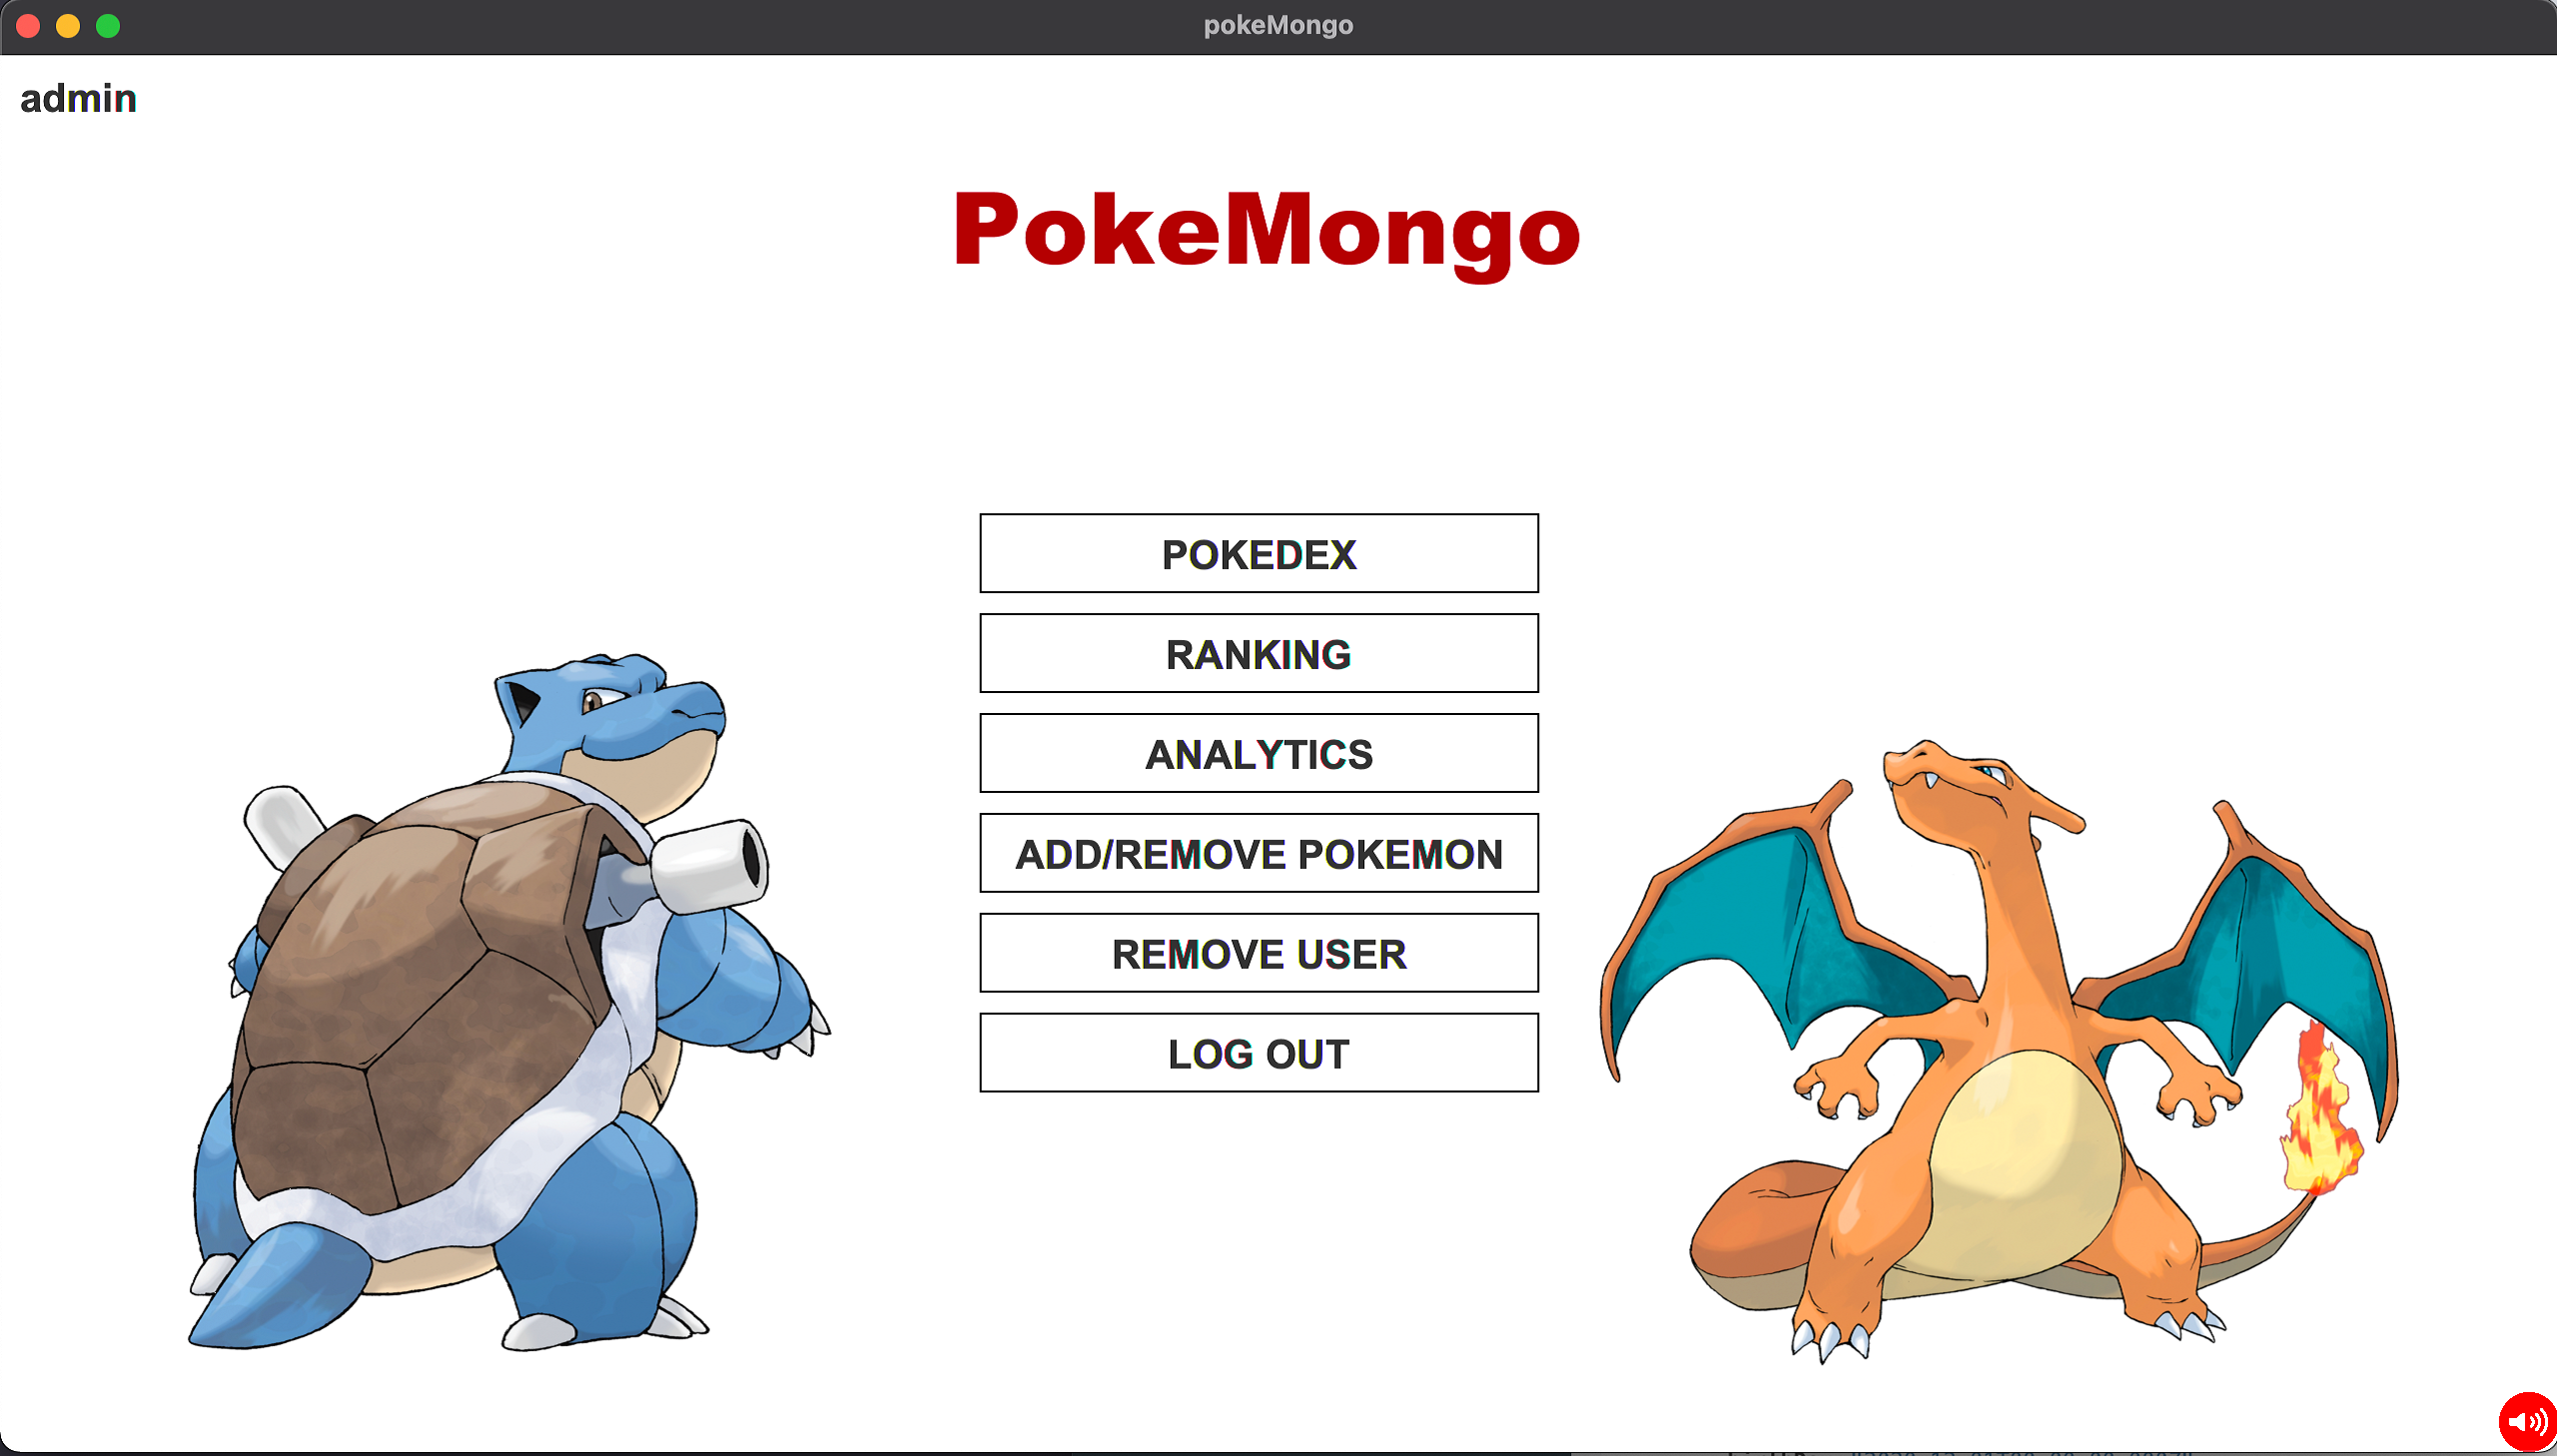
\includegraphics[width=\textwidth]{img/userManual/admin_homepage.png}
	\caption{Admin Homepage}
\end{figure}
Notice that the \textit{Pokedex page} and the \textit{Ranking page} are the same as the Normal User, with some slightly differences. Furthermore, the number of \textit{daily pokeballs} is not present, due to the fact that the admin could not play the catch'em all game, because it would be unfair (the Admin can ban Users or delete Pokemons).

\subsubsection{Differences with Normal User}
By opening the \textit{Team Information Popup} the admin has the possibility to delete some \textbf{Posts} or \textbf{Replies} as shown in the following figure, in which are presents some \textbf{DELETE labels} in each \textbf{Post} or \textbf{Reply}.
\begin{figure}[H]
	\centering
	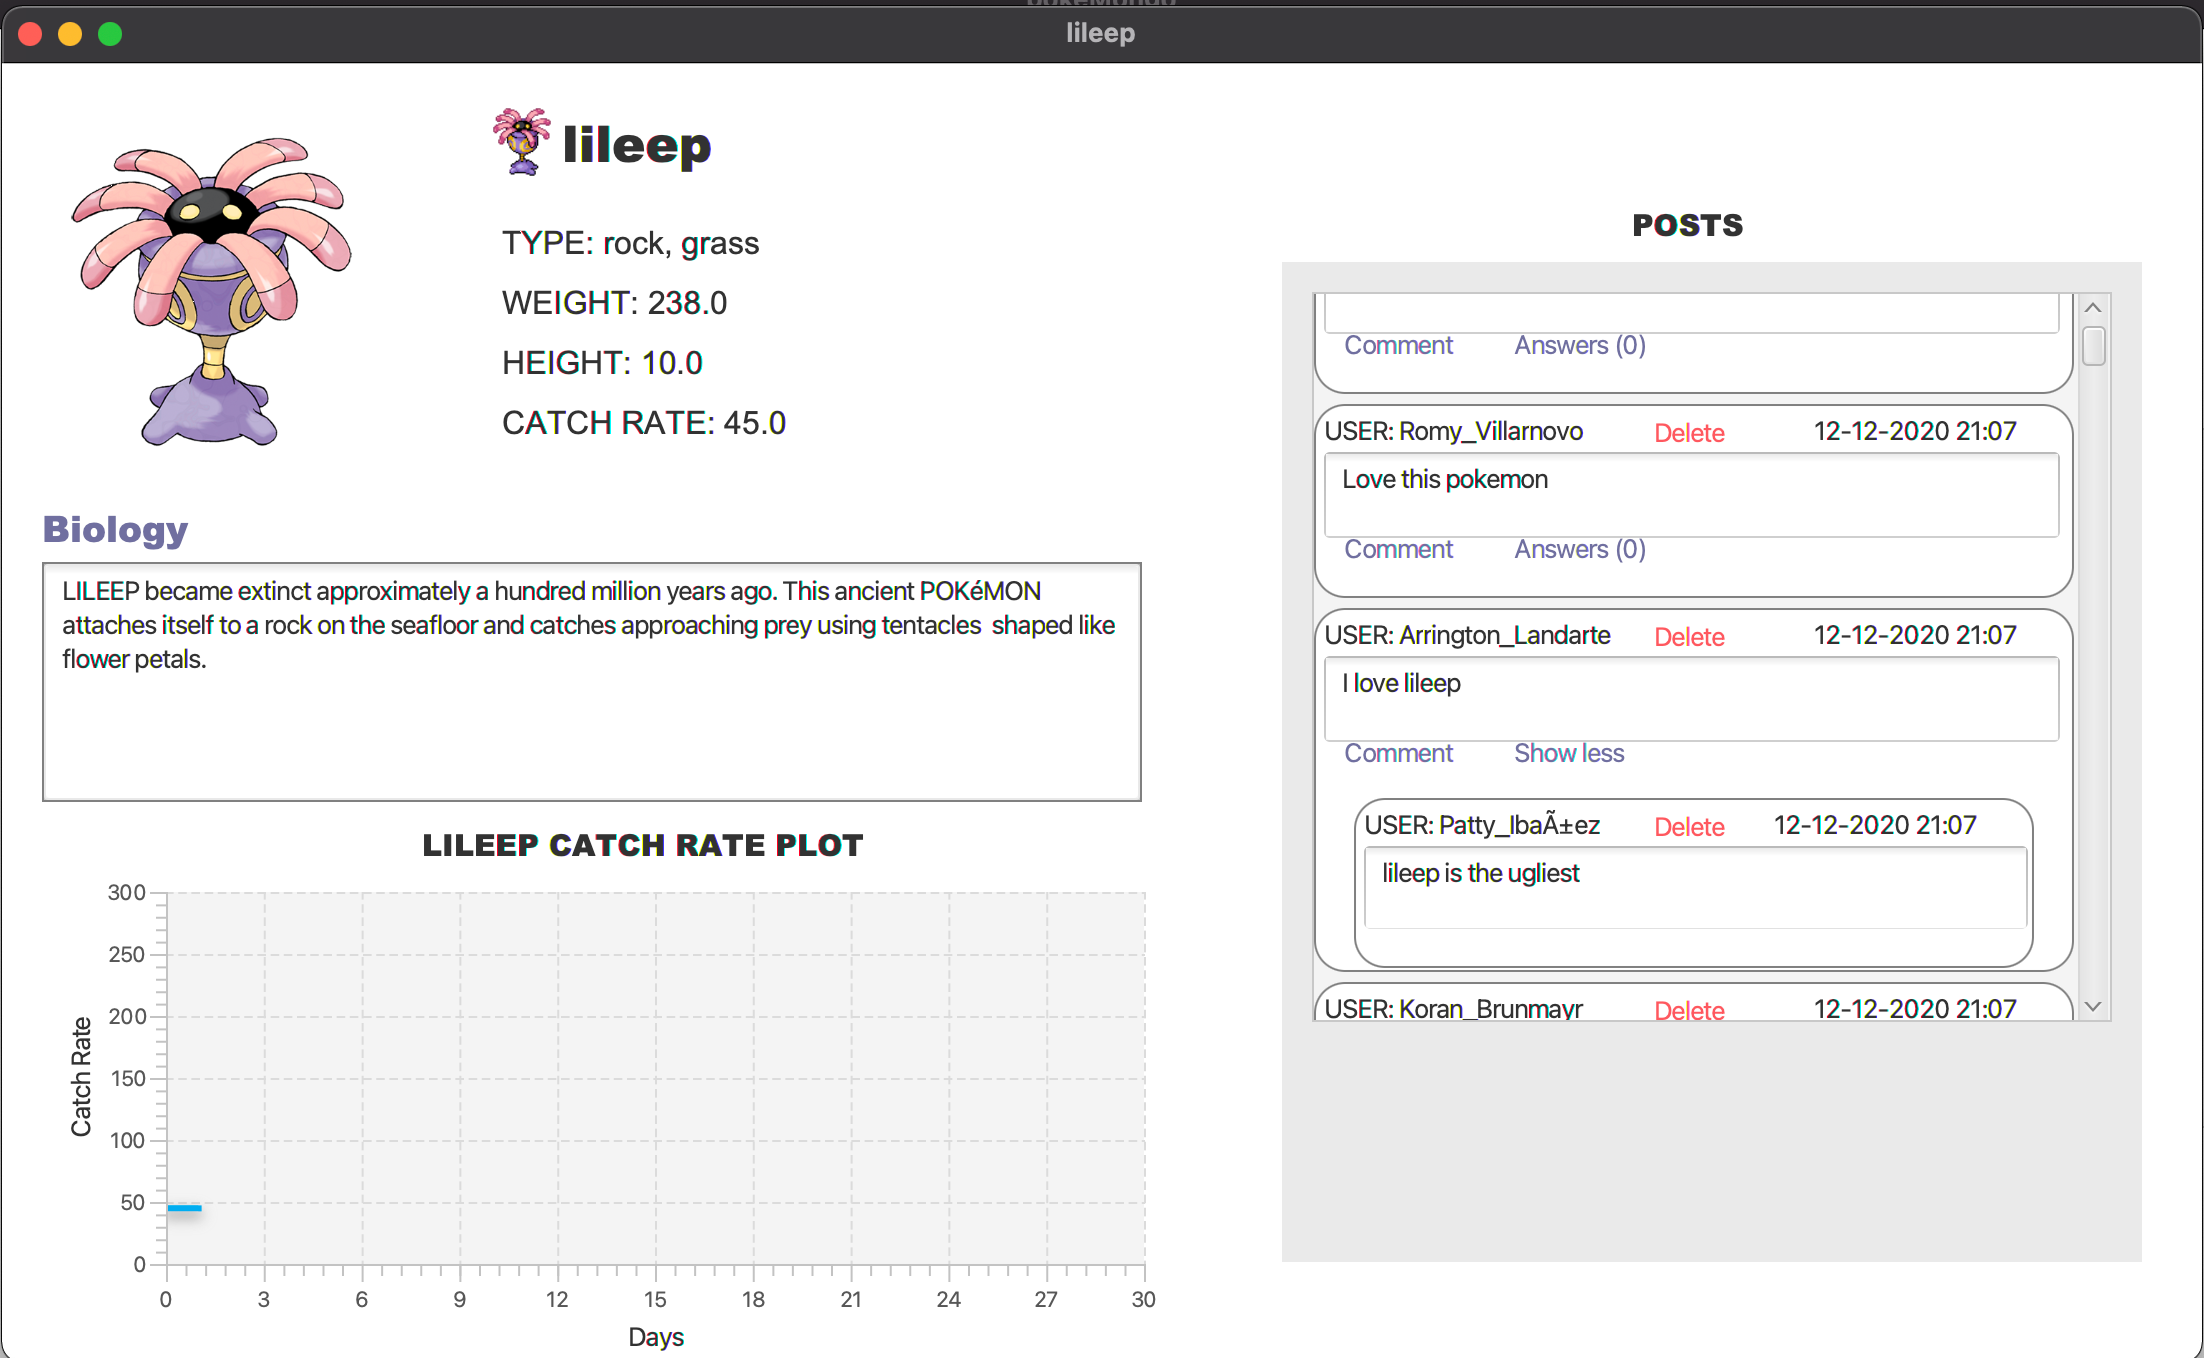
\includegraphics[width=\textwidth]{img/userManual/admin_pokemon_window.png}
	\caption{Admin Pokemon Popup}
\end{figure}
Moreover, in the \textit{Ranking page}, there is no ranking among friends because the admin can not have friends (FOLLOWING) or be friend (FOLLOWER) of someone.

\subsubsection{Analytics}
In the following page the \textbf{Admin} can have some insights about the usage statistics of the application. In fact, in the top-left plot, there is plotted the number of total \textbf{User} in the last 30 days. On the bottom-left there is another plot with the number of daily logins in the last 30 days.
On the right there is a similar plot, which can be filtered by \textit{Country} through the apposite combobox.
\begin{figure}[H]
	\centering
	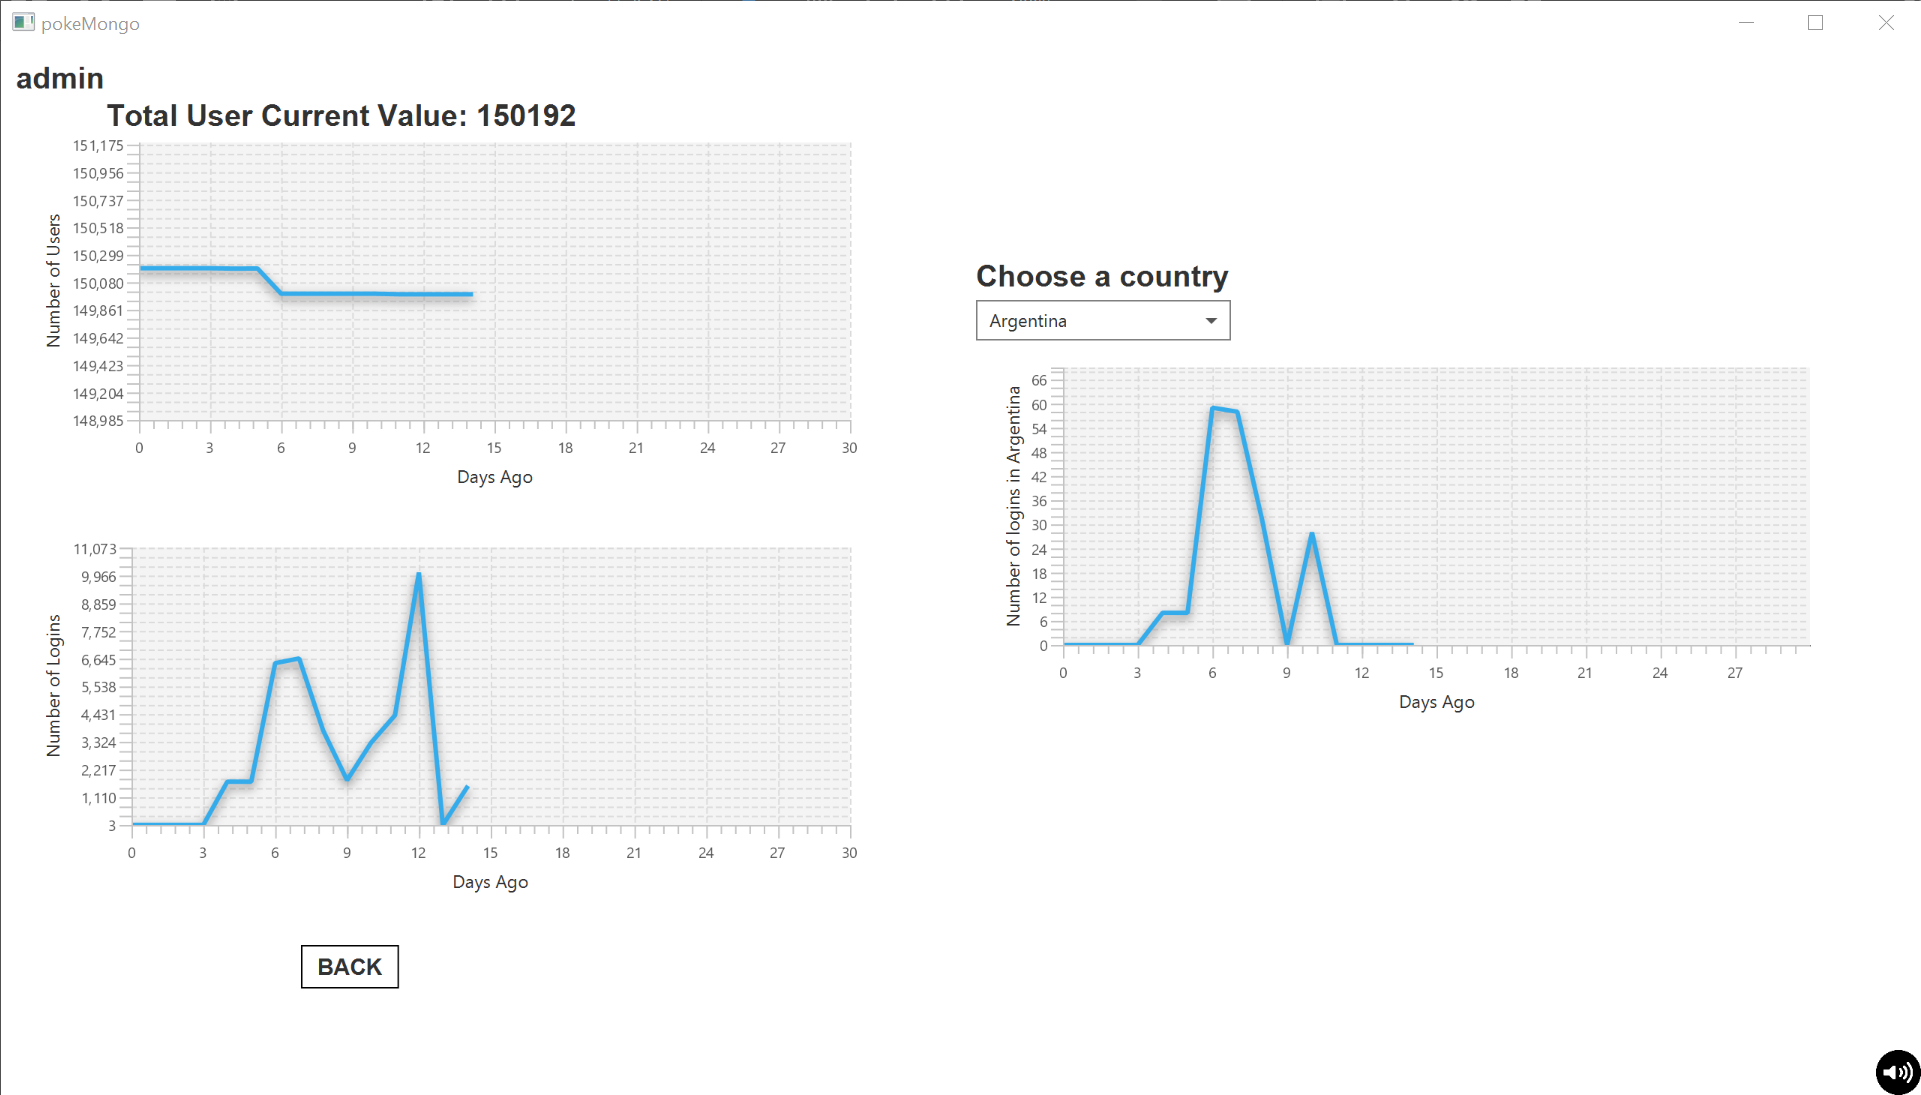
\includegraphics[width=\textwidth]{img/userManual/usage_statistics.png}
	\caption{Analytics Page}
\end{figure}

\subsubsection{Add/Remove Pokemon}
In this page, by clicking on one of the radio buttons on the top, is possible to delete or add a \textbf{Pokemon} in the system in order to update the application if there are some new \textbf{Pokemons} released by GameFreak or just some fan-made ones. 
In order to add a \textbf{Pokemon}, after selecting the \textbf{radio button ADD POKEMON}, the \textbf{Admin} must compile every field of the form, by adding even the urls of the images that will be shown. Then, he must \textit{click} the \textbf{ADD button} and a green popup will be shown if the procedures have been made correctly. 
\begin{figure}[H]
	\centering
	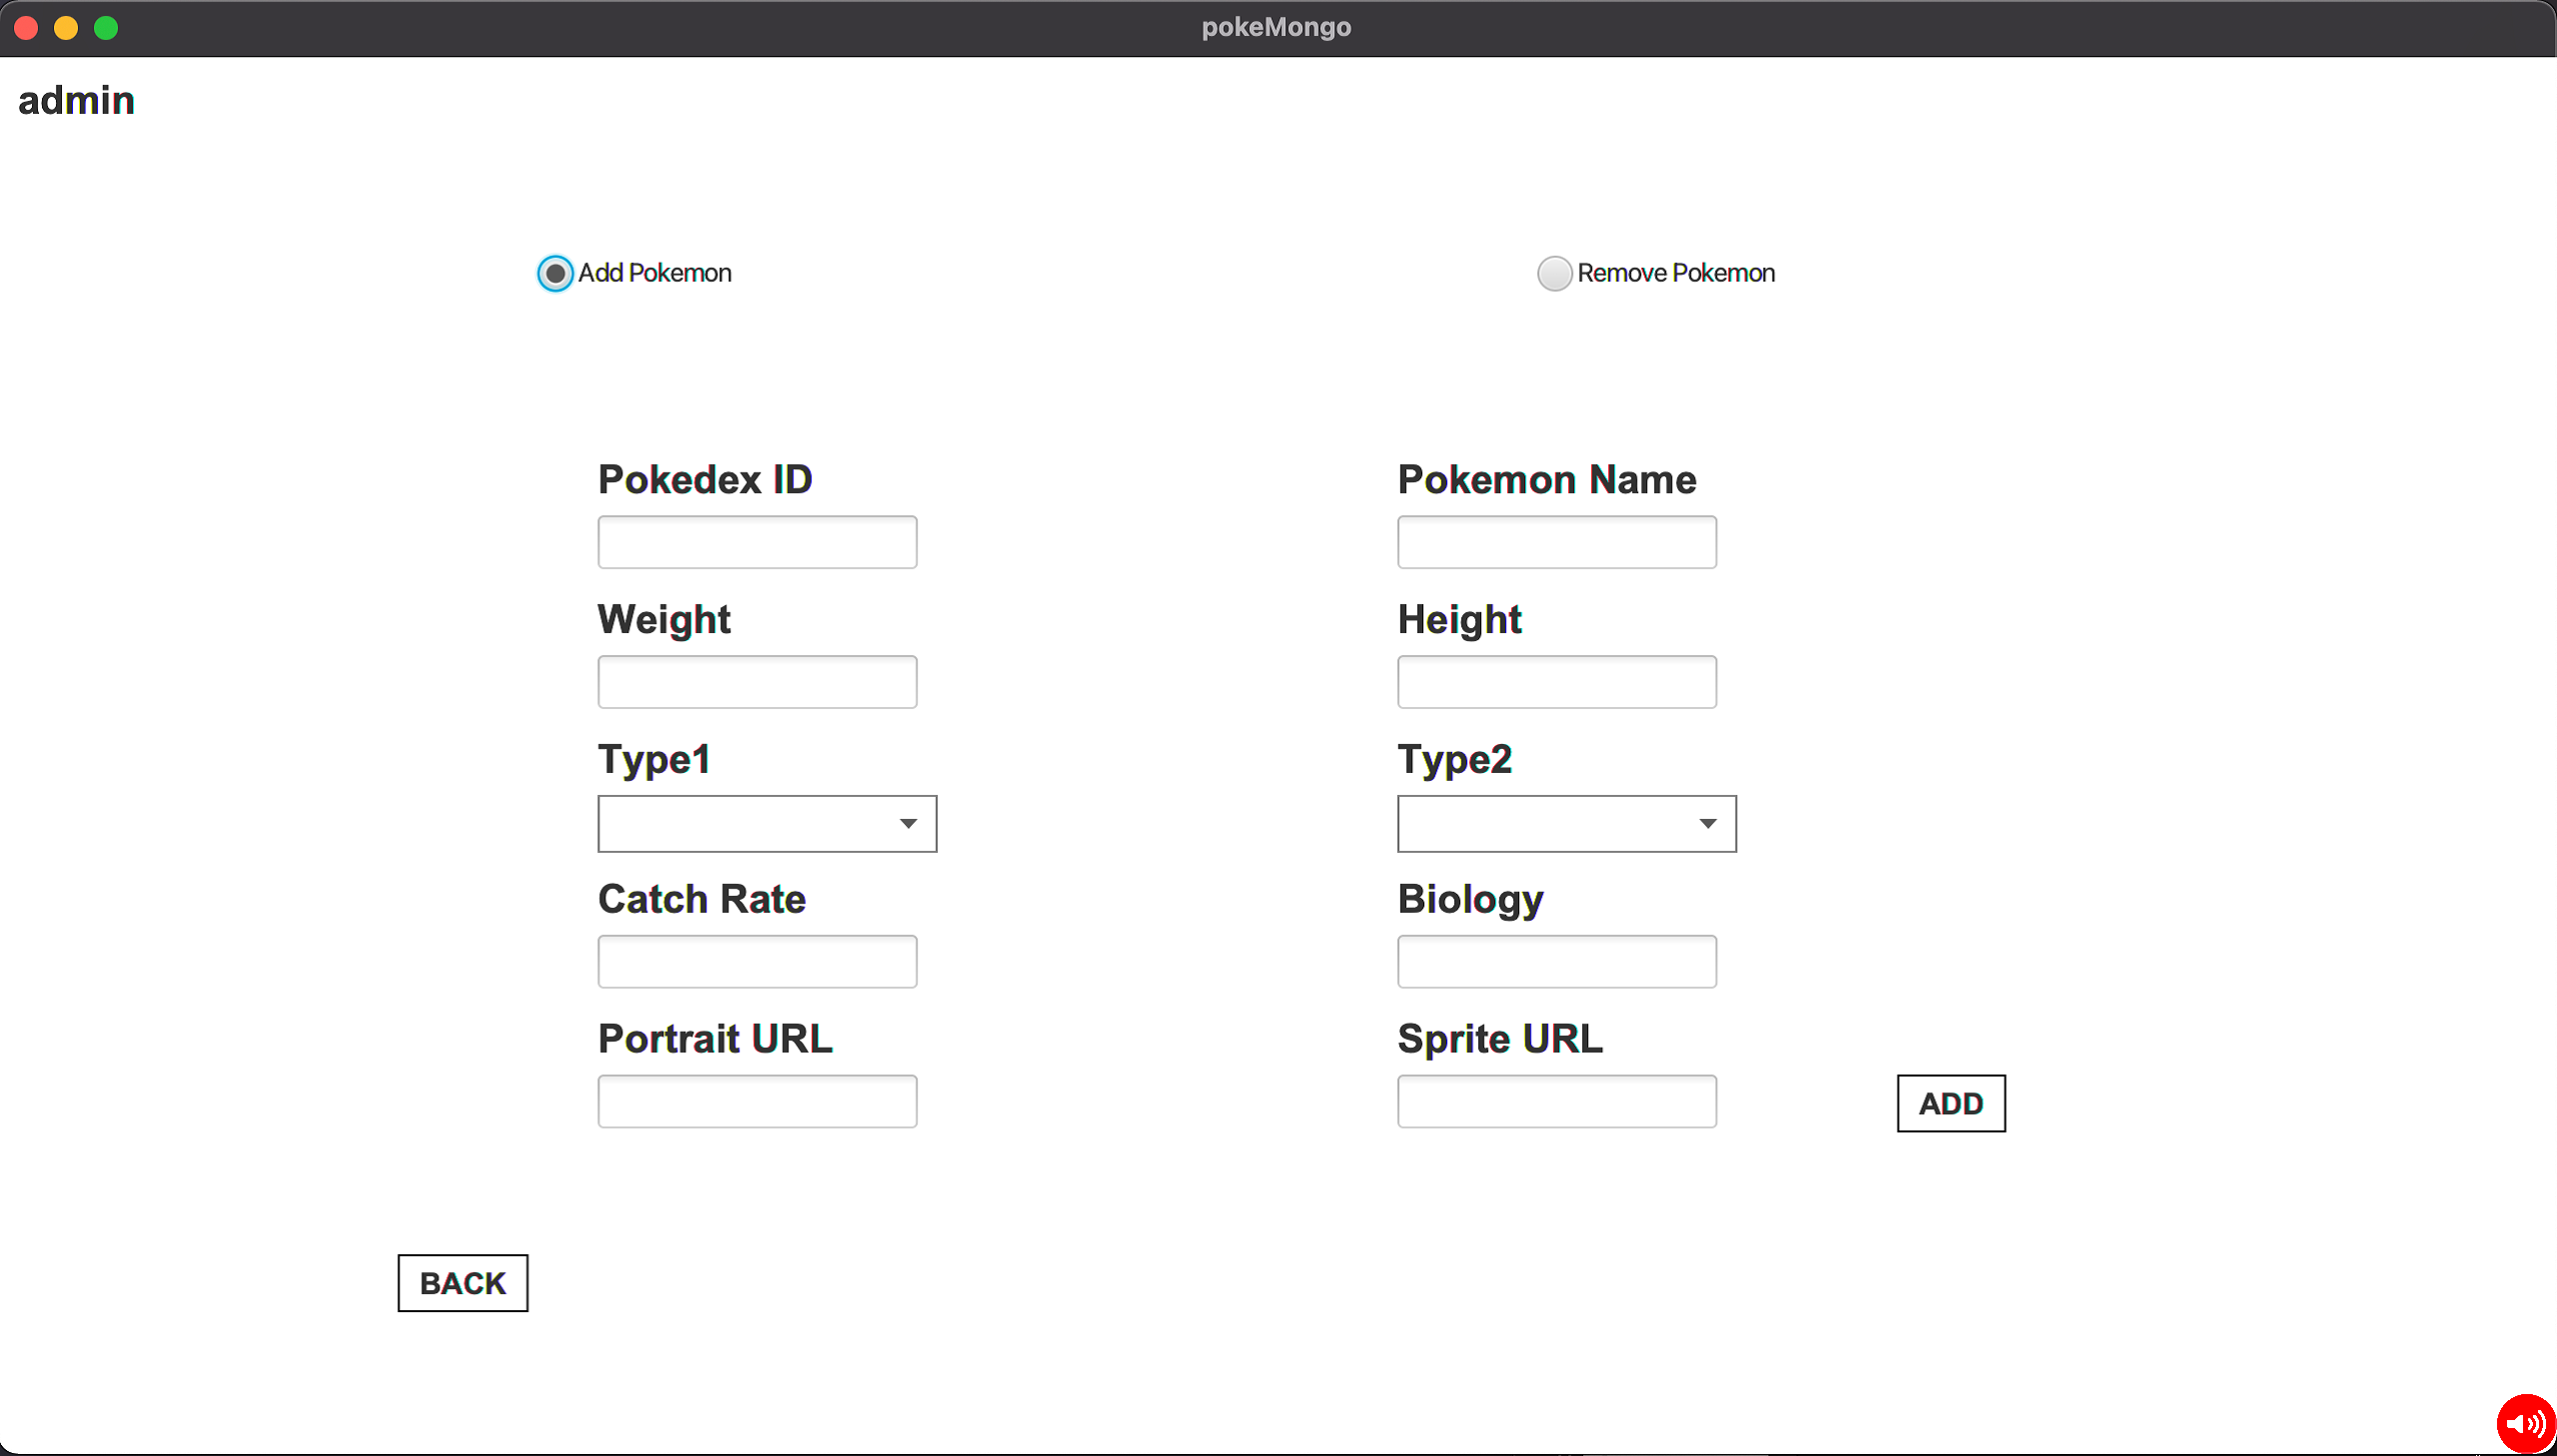
\includegraphics[width=\textwidth]{img/userManual/add_pokemon.png}
	\caption{Add Pokemon Page}
\end{figure}
For removing a \textbf{Pokemon} is enough to write down the \textit{pokemon name} and \textit{click} the \textbf{REMOVE button}, a green popup will be showed in order to confirm the deletion.
\begin{figure}[H]
	\centering
	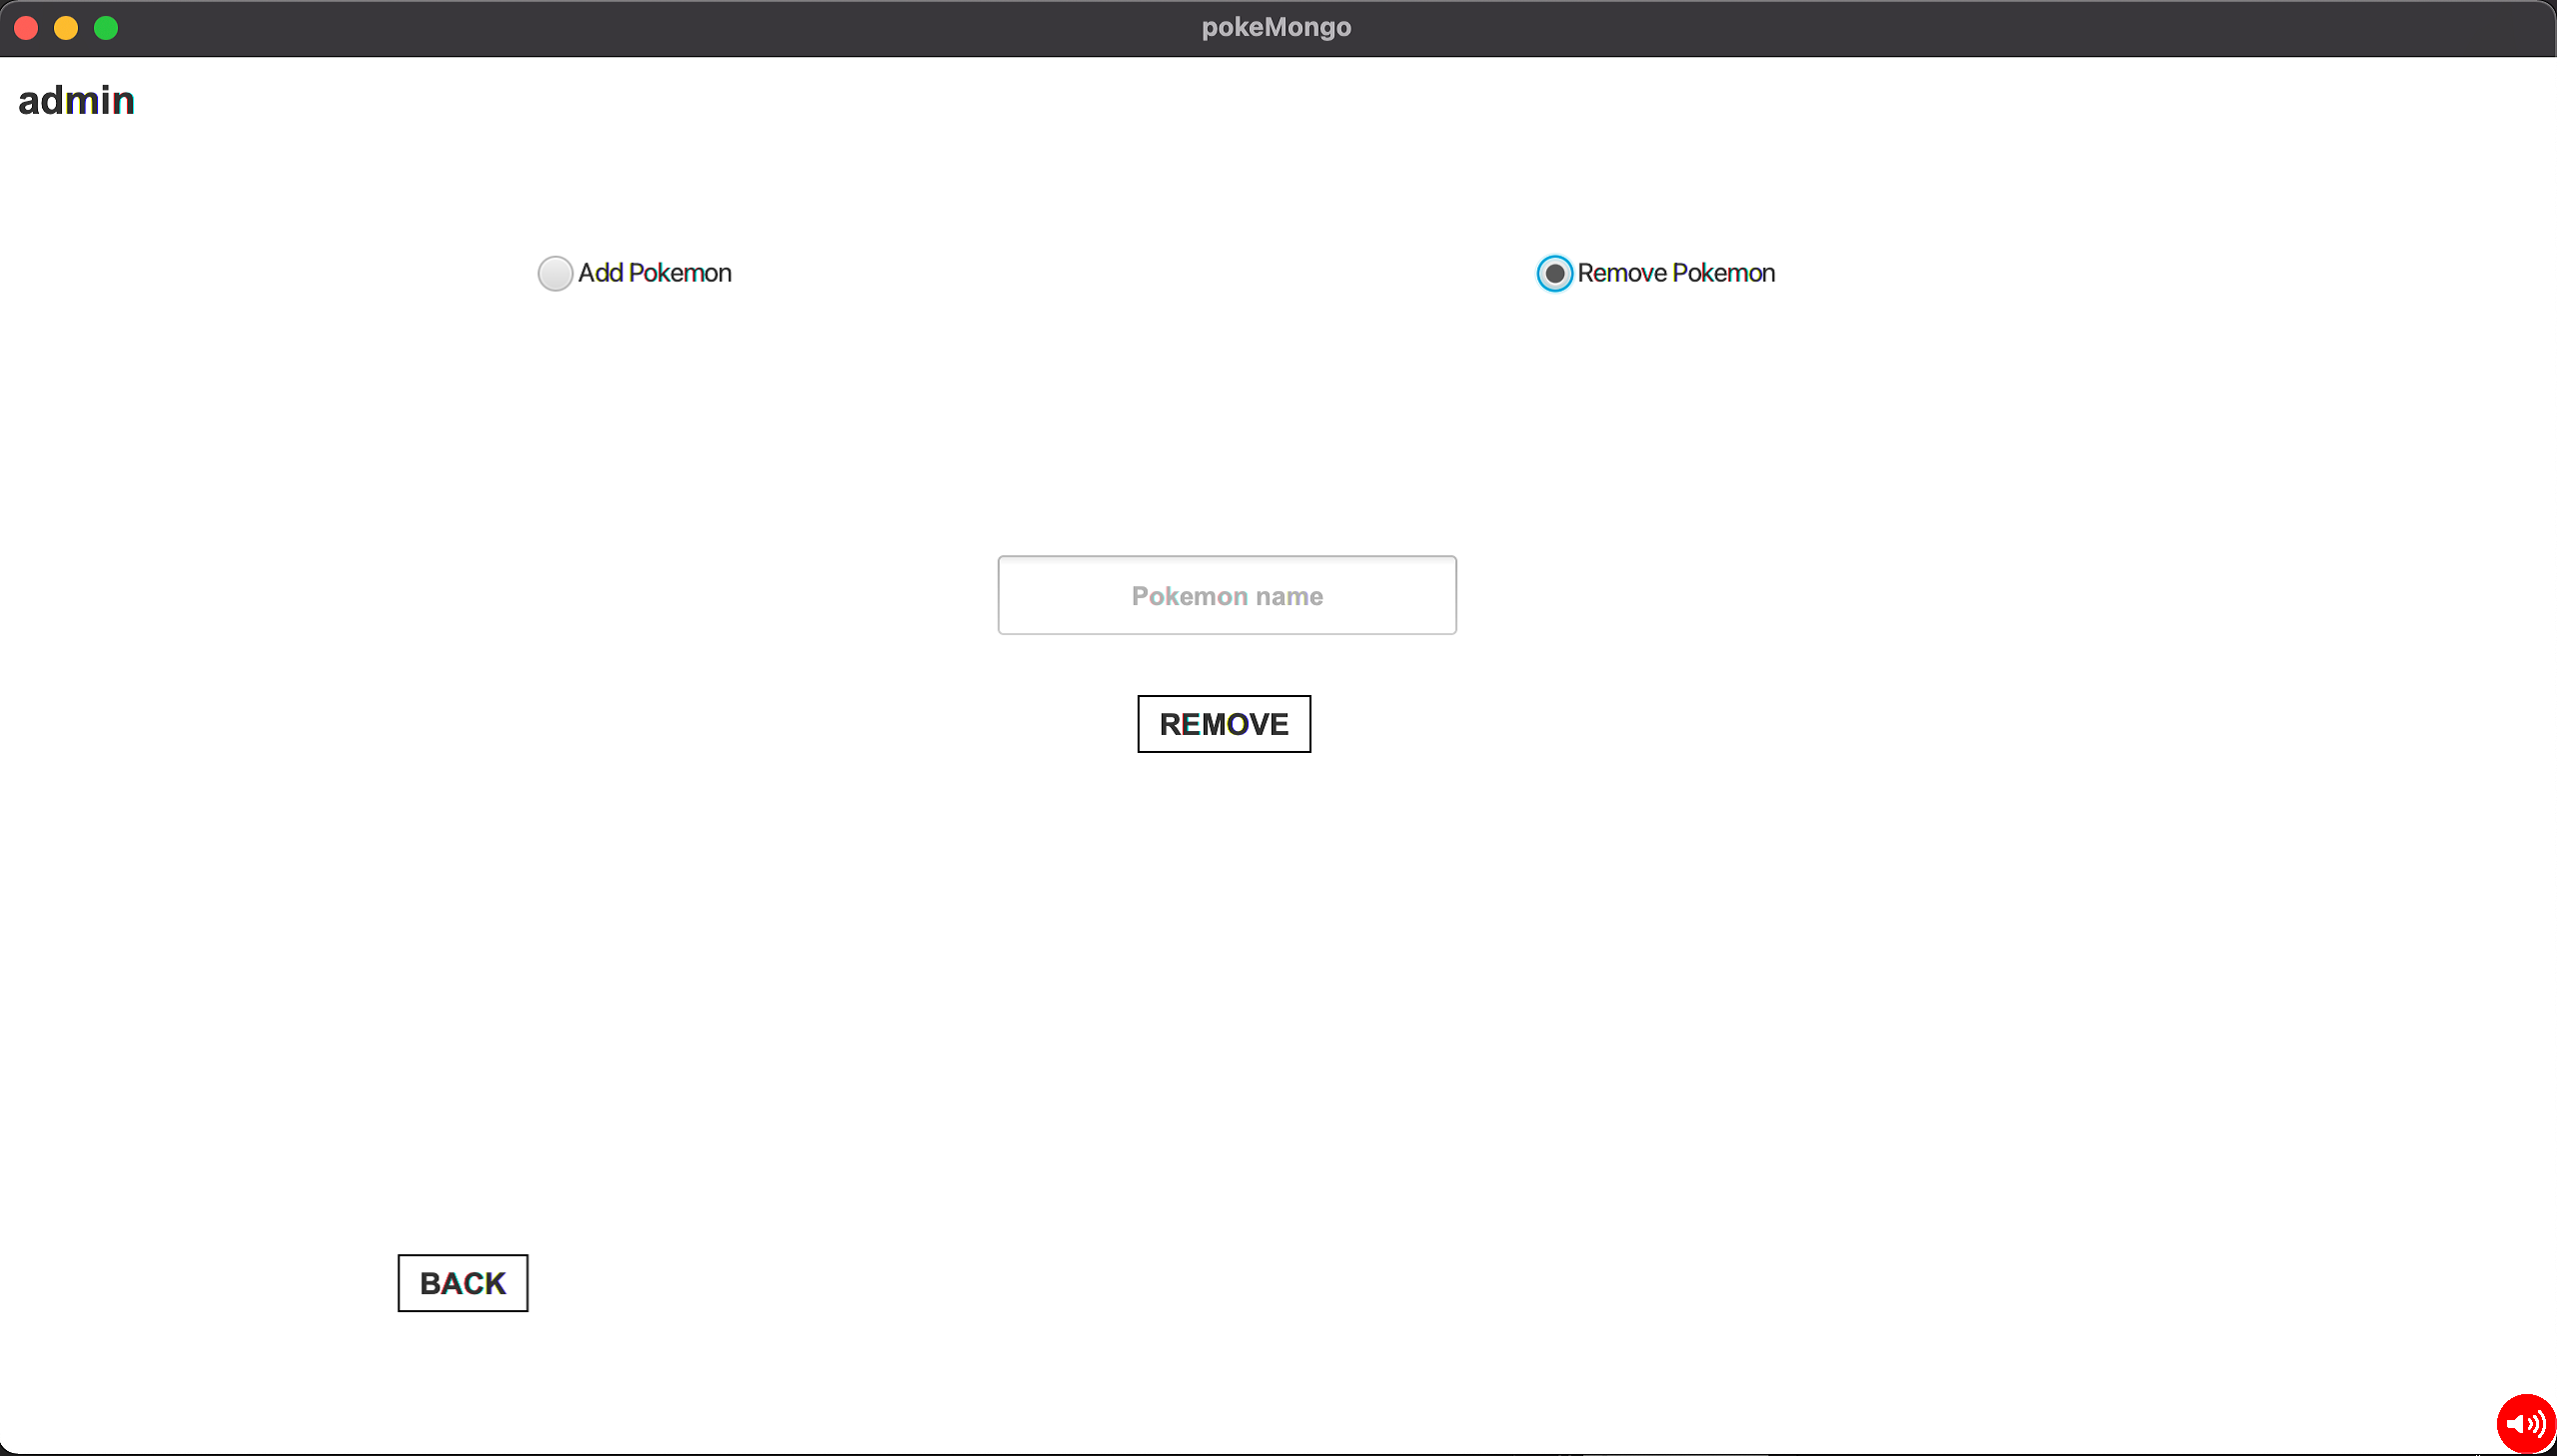
\includegraphics[width=\textwidth]{img/userManual/remove_pokemon.png}
	\caption{Remove Pokemon Page}
\end{figure}
\subsubsection{Remove Users}
An \textbf{Admin} can decide to ban a mischievous \textbf{User}. In order to do so, there is the \textit{Delete User Page} in which, by just typing the \textit{username} of that particular \textbf{User} and pressing the \textbf{REMOVE button}, the \textbf{User} will be removed from the system. If a green popup will be displayed, it will mean that the \textbf{User} deletion operation has been completed successfully. 
\begin{figure}[H]
	\centering
	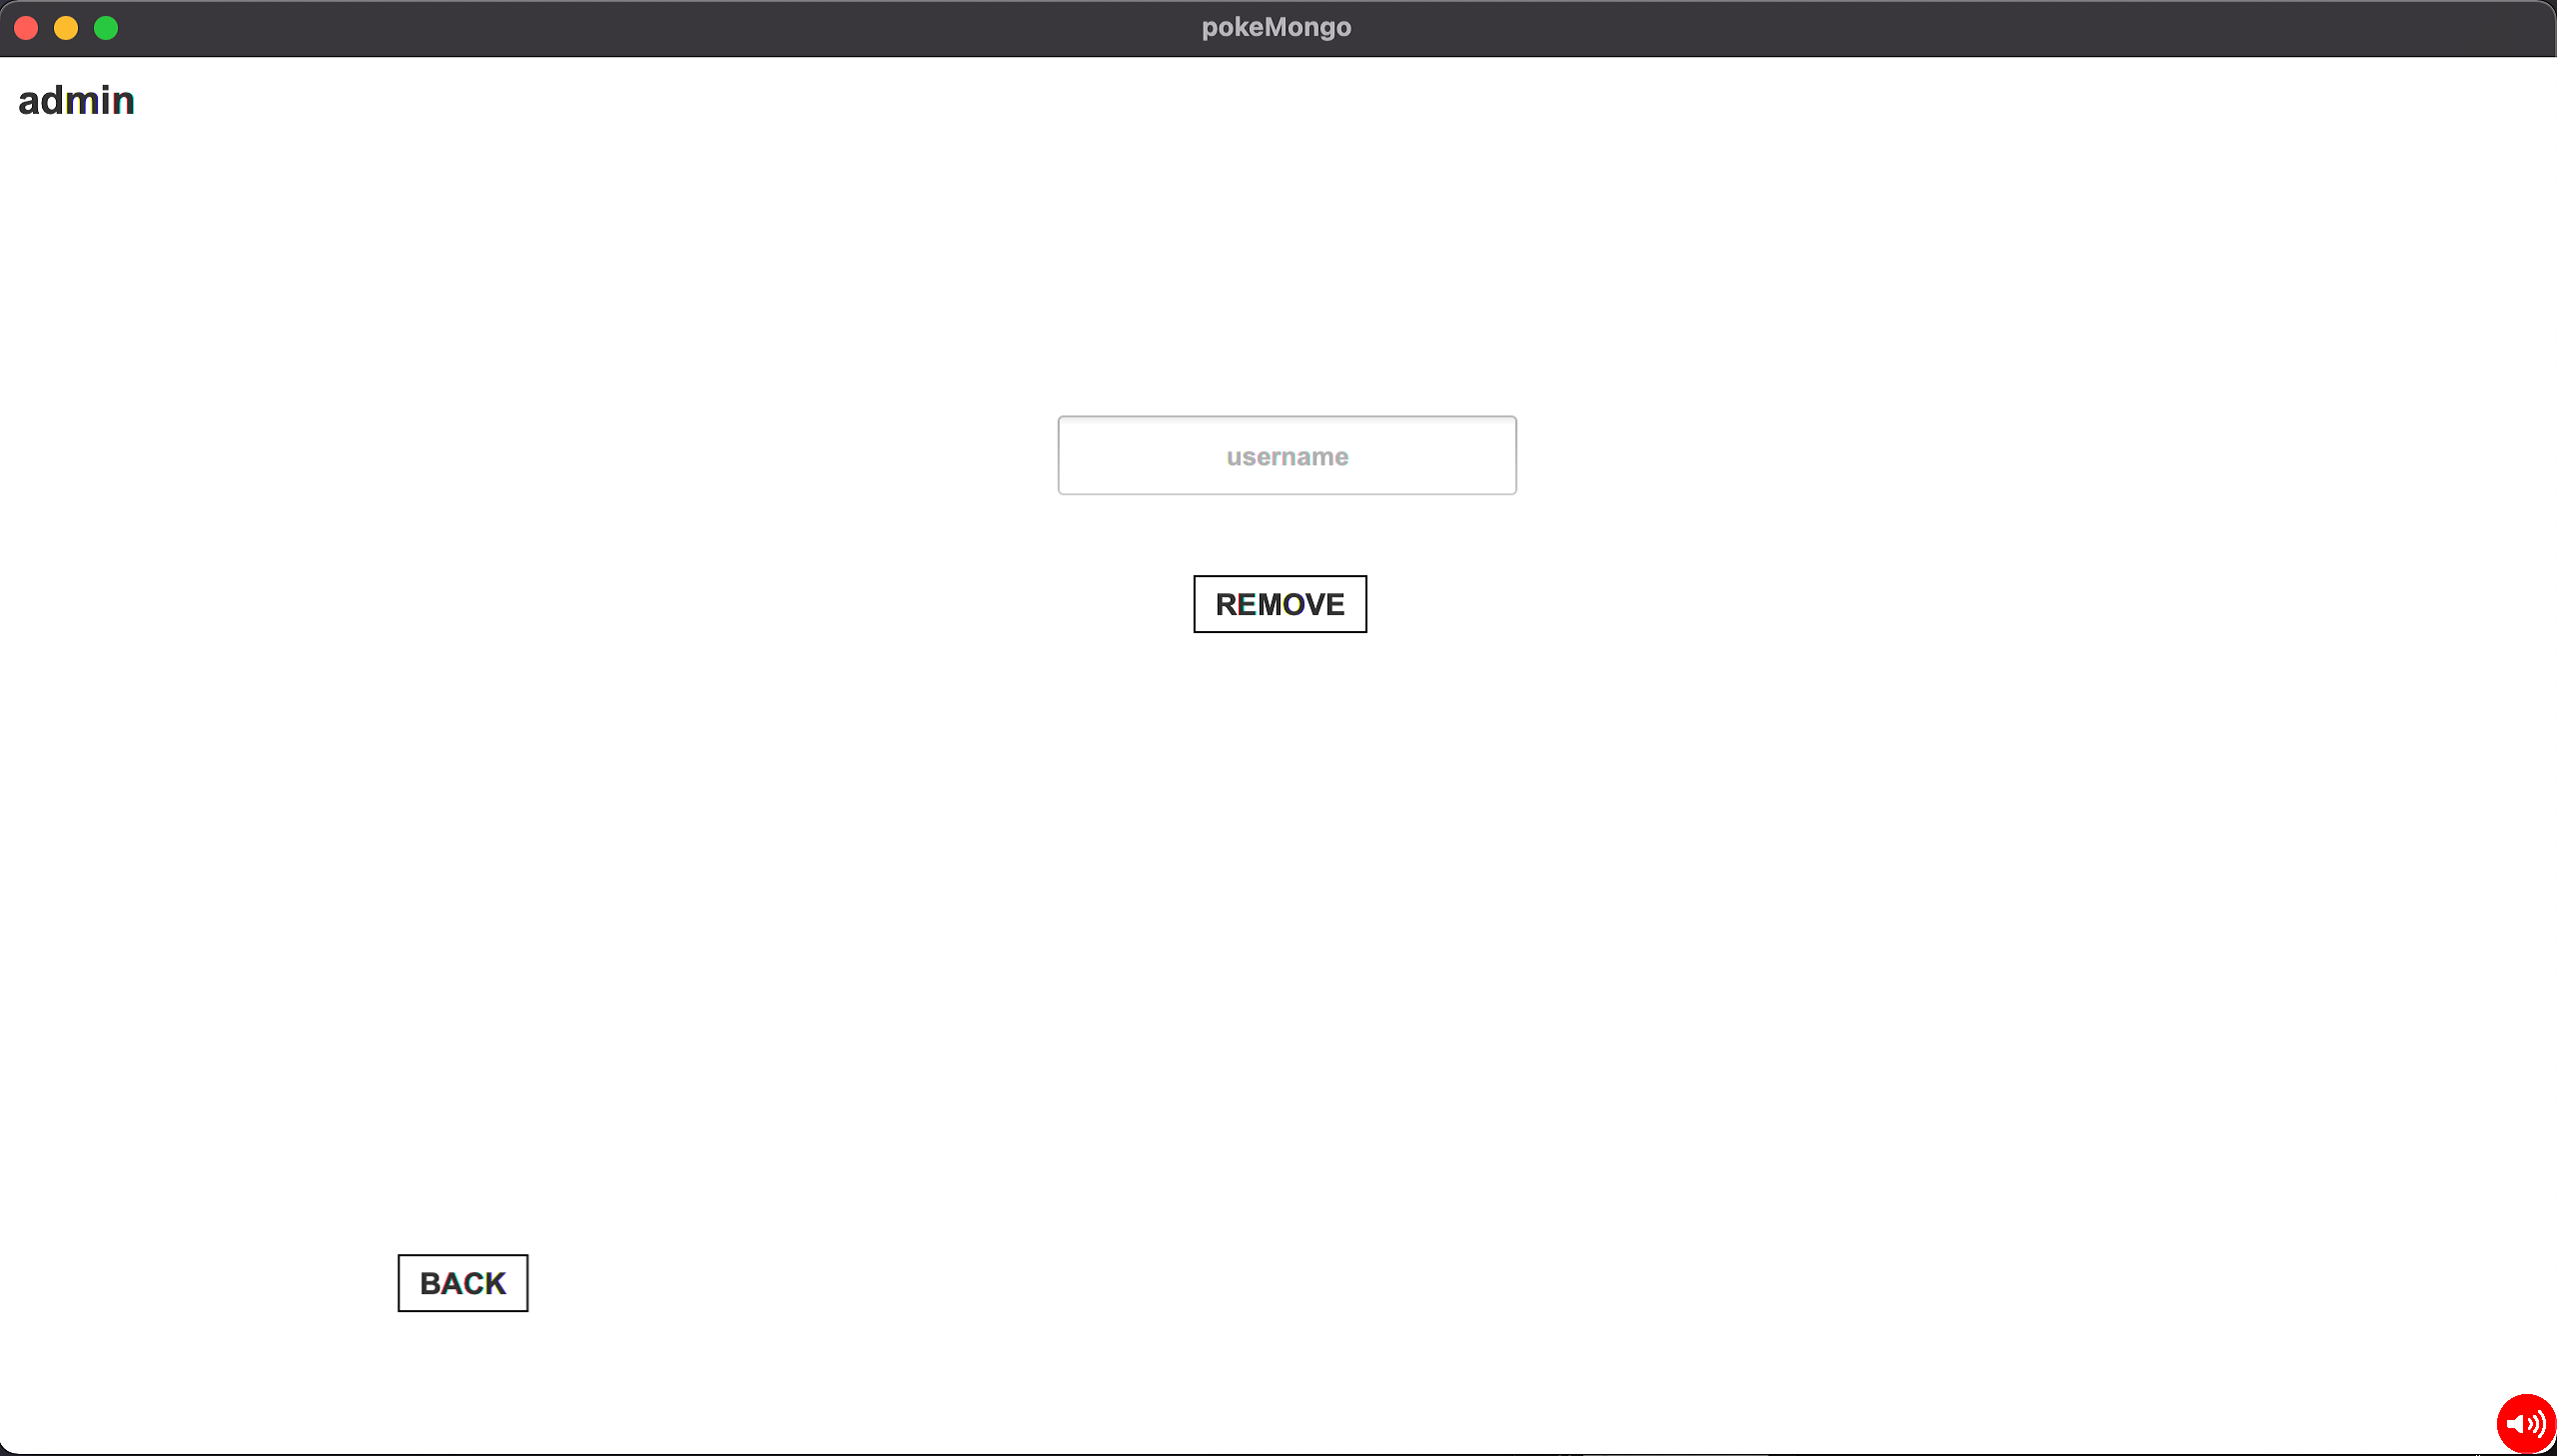
\includegraphics[width=\textwidth]{img/userManual/delete_user.png}
	\caption{Delete User Page}
\end{figure}